\chapter{Background}\label{chap:background}

\section{Data Spaces and the IDS Initiative}\label{sec:data-spaces-ids}

A dataspace is, in the standardised formulation of ISO/IEC~FDIS~20151-1, ``an environment enabling trusted data sharing between participating parties, based on agreed governance framework, along with agreed set of policies, semantic models, standardised protocols, processes, and facilitating services''~\citep{isoiec20151, idsaknowledgebase}. The definition is deliberately negative as much as positive: it tells implementers what a dataspace is \emph{not}. It is not a data lake, in which storage is consolidated; not a data warehouse, in which schemas are imposed top-down; and not a hyperscaler platform, in which a single operator controls the substrate~\citep{designingdataspace}. The dataspace pattern instead distributes storage and authority across independent participants who exchange data peer-to-peer under shared rules~\citep{idsaknowledgebase, IDS4.0}. The European data strategy frames this distribution as a precondition for a single market for data in which participants retain sovereignty over what they share, with whom, and under what terms~\citep{europeancommission2020}.

Three structural elements recur in every operational dataspace and provide the vocabulary for the rest of this thesis. \emph{Participants} are organisations that produce or consume data and that ``follow common rules defined in the data space's governance framework''~\citep{idsaknowledgebase}. A \emph{Data Space Governance Authority} establishes, governs, and enforces those rules; the authority ``may be provided by one or more parties, in a centralized or decentralized manner''~\citep{idsaknowledgebase}. Each participant is technically represented by a \emph{connector}, a software agent that ``acts on behalf of [the] organization in the data space'' and exposes the \gls{api} endpoints for discovery, contract negotiation, and data exchange~\citep{idsaknowledgebase}. \Cref{fig:dataspace-overview} sketches these elements inside a single dataspace, together with the supporting services for identity, vocabularies, and observability.

\begin{figure}[ht]
    \centering
    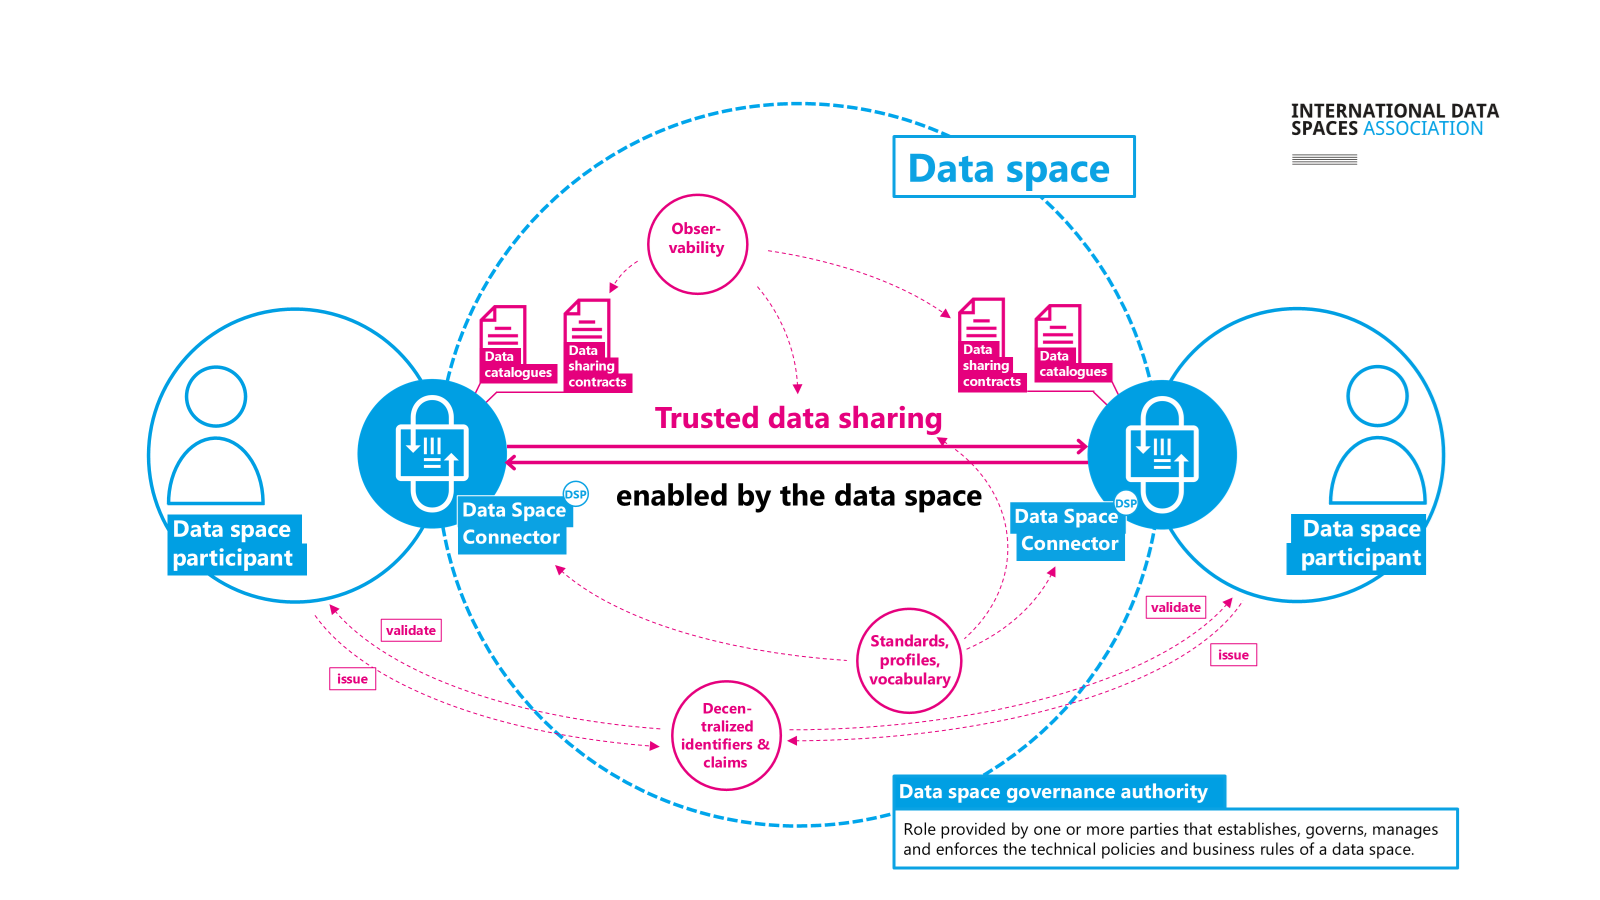
\includegraphics[width=0.85\linewidth]{figures/dataspace_overview.png}
    \caption[Structural elements of a single dataspace]{Structural elements of a single dataspace: participants, connectors, the Data Space Governance Authority, and the supporting services for identity, vocabularies, and observability. Figure source: International Data Spaces Association.}
    \label{fig:dataspace-overview}
\end{figure}

\newpage

The International Data Spaces Association (IDSA) is the standards organisation that has carried this model from concept to specification. Its Manifesto articulates the design principles that constrain every downstream component, including the connectors evaluated in this thesis: ``actors shall have full autonomy in deciding with whom they share data with and under what conditions'' (sovereignty); ``data does not flow through the dataspace'' but on private peer-to-peer channels (decentralised exchange); ``dataspaces shall be infrastructure agnostic'' (no single platform); and ``unity in standards~--~freedom in implementation'' (a common specification realised by diverse implementations)~\citep{idsaknowledgebase}. The last principle is what makes this thesis possible: multiple connector implementations claim conformance to the same specification, and their relative performance is therefore a meaningful research question. IDSA realises these principles through two specifications used throughout this thesis: the IDS Reference Architecture Model~\citep{IDS4.0} and, jointly with the Eclipse Dataspace Working Group, the Dataspace Protocol~\citep{datapsaceProtocol2025}.


\subsection{International Data Spaces Reference Architecture}\label{subsec:ids-ram}

The \emph{IDS Reference Architecture Model} (IDS-RAM)\glsadd{idsram}, currently in its fourth edition, is an abstract architecture rather than an implementation~\citep{IDS4.0}. It resides at a higher abstraction level than common architecture models of concrete software solutions and is meant to be instantiated by independent implementers~\citep{IDS4.0, otto2019ids}. 
\newpage
The model is organised as five horizontal layers crossed by three cross-cutting perspectives, as shown in \Cref{fig:ids-ram-overview}; this structure recurs verbatim in the documentation of every connector evaluated in \Cref{chap:results-evaluation}.

\begin{figure}[ht]
    \centering
    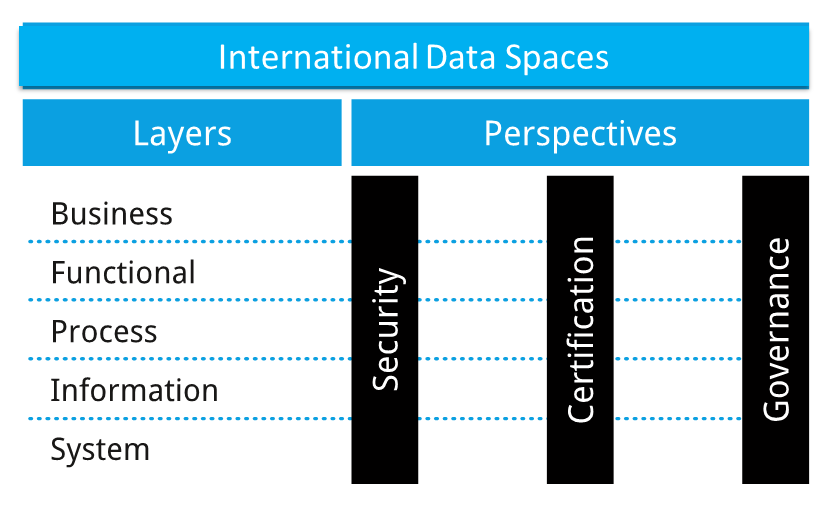
\includegraphics[width=0.78\linewidth]{figures/ids_ram_overview.png}
    \caption[Overview of the IDS Reference Architecture Model]{Overview of the IDS Reference Architecture Model: five horizontal layers (Business, Functional, Process, Information, System) cross-cut by three perspectives (Security, Certification, Governance). Figure from the IDS-RAM~4 documentation~\citep{IDS4.0}, licensed under CC BY~4.0.}
    \label{fig:ids-ram-overview}
\end{figure}

The five layers move from organisational concerns to technical realisation~\citep{IDS4.0, otto2019ids}. The \textbf{Business Layer} ``specifies and categorizes the different roles which the participants of the International Data Spaces can assume'' and the interaction patterns between them, including the contractual basis of usage policies. The \textbf{Functional Layer} defines the functional requirements of the IDS across concern areas of which trust, security, and data sovereignty are the most load-bearing for connector design. The \textbf{Process Layer} describes the dynamic interactions between components using BPMN; this layer is where the asynchronous sequence of catalog request, contract negotiation, and transfer initiation becomes explicit, and \Cref{sec:dsp} returns to it. The \textbf{Information Layer} defines a linked-data conceptual model for both static metadata (catalog entries, policy expressions) and dynamic state (contract agreements, transfer-process records). The \textbf{System Layer} concerns the decomposition of the logical software components, considering integration, configuration, deployment, and extensibility~\citep{IDS4.0}~--~this is the layer at which an EDC, a Tractus-X EDC, a Factory-X EDC, a DSP-Native BaSyx connector, or the Fraunhofer ISST EDC are distinguishable from one another.

Three cross-cutting \emph{perspectives} apply at every layer~\citep{IDS4.0}: \textbf{Security} (cryptographic identities, message integrity, confidentiality of in-transit and at-rest data), \textbf{Certification} (third-party assurance that a participant or component meets the IDS criteria), and \textbf{Governance} (the policies under which the dataspace as a whole is operated and audited). Of these, the Security perspective has the most direct performance footprint, because identity verification and policy evaluation are on the critical path of every contract negotiation and transfer-process initiation; \Cref{chap:results-evaluation} returns to that observation when interpreting the measured results.

The Business Layer further enumerates roles that recur in the source code of every connector reviewed in \Cref{sec:connectors}. The most relevant to this thesis are the \textbf{Data Provider} and \textbf{Data Consumer}, the two endpoints of a transfer; the \textbf{Identity Authority}, which ``offer[s] a service to create, maintain, manage, monitor, and validate identity information of and for participants''~\citep{IDS4.0}; the \textbf{Vocabulary Intermediary}, which manages the ontologies used in catalog descriptions; the \textbf{Clearing House}, which ``provides clearing and settlement services for all financial and data exchange transactions'' and so anchors non-repudiation~\citep{IDS4.0}; and the \textbf{Connector Developer}, ``[providing] software for implementing the functionality required by the International Data Spaces''~\citep{IDS4.0}~--~the role this thesis evaluates. \Cref{fig:ids-ram-roles} shows how these roles interact through three distinct flows~--~data, metadata, and software~--~routed via the intermediaries; the diagram makes explicit that no actor short-circuits the Clearing House for transaction logging, and that vocabularies are pushed to providers and consumers in parallel rather than embedded in the data flow itself.

\begin{figure}[ht]
    \centering
    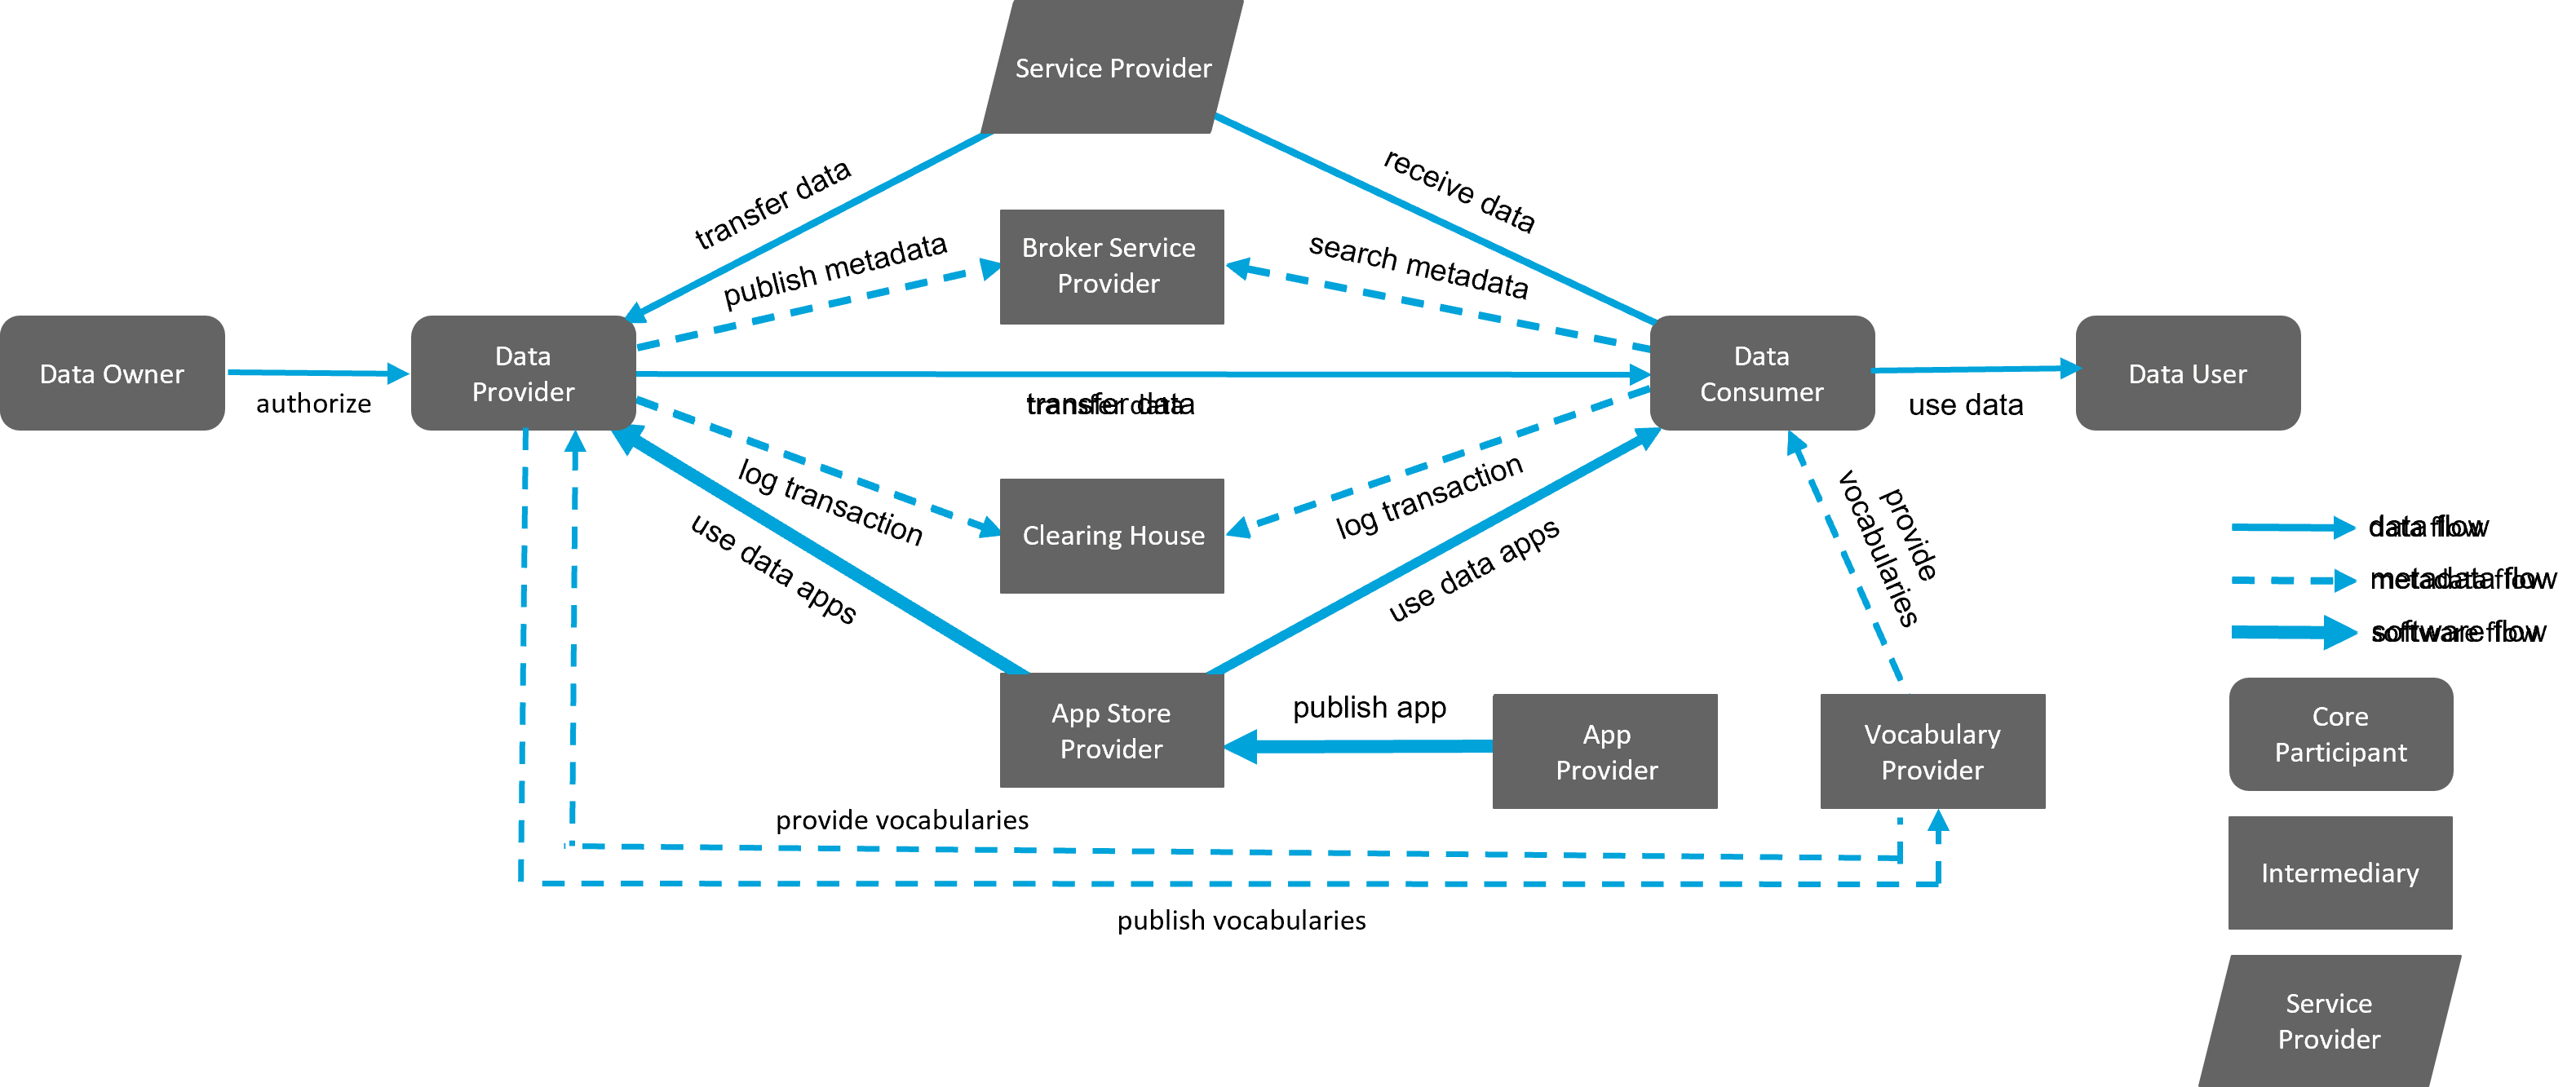
\includegraphics[width=0.95\linewidth]{figures/ids_ram_roles_interactions.png}
    \caption[Roles and interactions in the International Data Spaces]{Roles and interactions in the International Data Spaces. Solid arrows denote data flow, dashed arrows metadata flow, and thick arrows software flow; Core Participants and Intermediaries are distinguished by node shape. Figure from the IDS-RAM~4 documentation~\citep{IDS4.0}, licensed under CC BY~4.0.}
    \label{fig:ids-ram-roles}
\end{figure}

The thesis-level consequence of this structure is straightforward. All four connectors in scope are System-Layer realisations of the same RAM. Their differences live primarily in how they instantiate the Functional Layer (identity provider, policy engine, transfer extensions) and how their System-Layer extensions are composed. The differences in measured throughput, latency, and resource consumption that \Cref{chap:results-evaluation} reports are therefore best read as the performance consequences of System- and Functional-Layer choices over a fixed Business- and Process-Layer specification.


\subsection{Gaia-X and Federated Data Ecosystems}\label{subsec:gaia-x}

\emph{Gaia-X} occupies a position adjacent to IDS rather than within it. Its stated mission is to become ``the \emph{de facto} standard to enable federated and/or decentralized and trusted data and infrastructure ecosystems''~\citep{gaiaxArchitecture}. Where IDSA specifies what a dataspace \emph{is} and how its participants exchange data, Gaia-X specifies the trust framework under which a participant~--~whether dataspace-affiliated or not~--~can be verified as compliant with a declared set of rules. The Gaia-X Architecture Document is explicit about this division: Gaia-X and IDSA ``deliver complementary technical frameworks'', with Gaia-X providing ``the decentralized digital trust framework'' and IDSA providing ``the Dataspace Protocol and the specific design concepts for data spaces''~\citep{gaiaxArchitecture}. Both align on the ISO/IEC~20151 dataspace definition introduced above~\citep{gaiaxArchitecture, isoiec20151}.

Federation in Gaia-X is achieved through two mechanisms rather than through a central authority~\citep{gaiaxArchitecture}. Ecosystems use ``the same language for specifying their trust model''~--~a shared, extensible ontology that the Architecture Document calls a ``\emph{lingua franca}''~--~and they agree on ``a common set of trusted ecosystem services'' such as identity providers, notaries, and assessment bodies. No single ecosystem owns these services; multiple ecosystems can adopt the same services voluntarily, and federation emerges from the overlap rather than from delegation. 

\newpage

This is the architectural basis on which two distinct dataspaces, each with its own governance authority, can negotiate data exchange across their boundary, as sketched in \Cref{fig:cross-dataspace}.

\begin{figure}[ht]
    \centering
    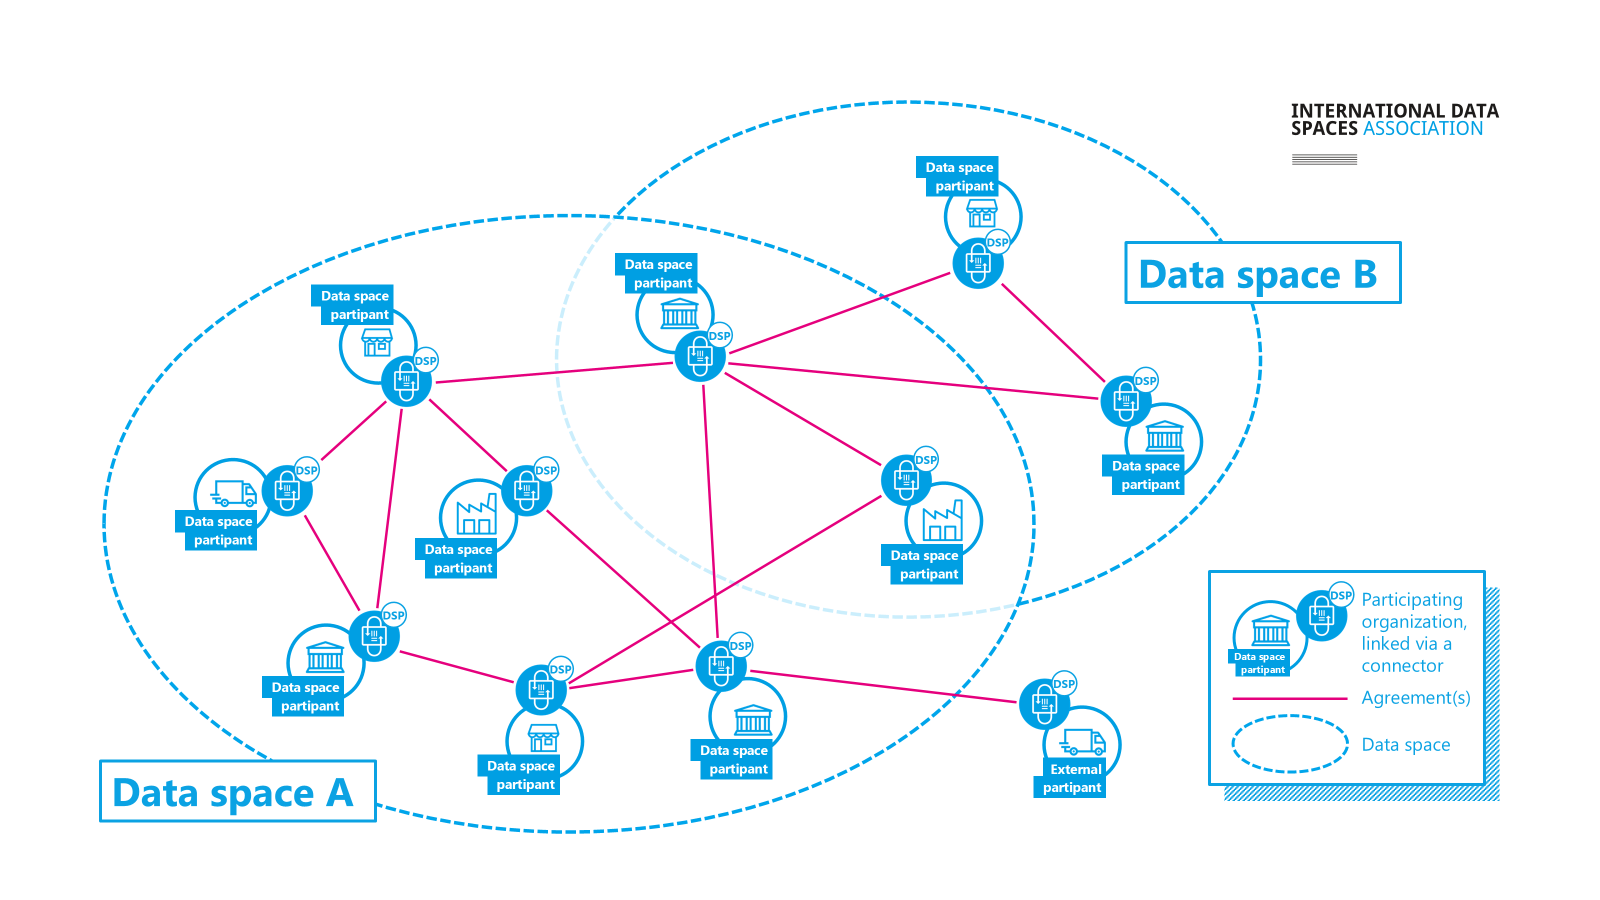
\includegraphics[width=0.85\linewidth]{figures/data_sharing_across_dataspaces.png}
    \caption[Cross-dataspace exchange between two dataspaces]{Cross-dataspace exchange: participants in Data Space~A and Data Space~B enter agreements mediated by their respective connectors, without consolidating storage in either dataspace. Figure source: International Data Spaces Association.}
    \label{fig:cross-dataspace}
\end{figure}

The trust framework is operationalised through machine-verifiable artefacts~\citep{GaiaXTrustFramework2024}. Participants, service offerings, and resources publish \emph{Self-Descriptions} that follow the W3C Verifiable Credentials Data Model, are ``cryptographically signed, preventing tampering with its content'', and are checked against computable rules that govern serialisation, signature validity, attribute consistency, and attribute veracity~\citep{GaiaXTrustFramework2024}. Compliance is therefore automated rather than negotiated case by case, which is what makes the framework scalable to multiple ecosystems with overlapping participants.

For the connectors evaluated in this thesis, the Gaia-X layer is not optional in production deployments. The Catena-X automotive dataspace and the Factory-X discrete-manufacturing dataspace both embed Gaia-X-aligned compliance into their participant onboarding and connector configuration~\citep{catenaxDocumentation}. In benchmarking terms this matters because a production-realistic connector deployment carries Gaia-X identity overhead in addition to DSP control-plane overhead, and the two cannot be cleanly separated without changing what is being measured. \Cref{chap:methodology} returns to this point when defining the measured workload, and \Cref{chap:results-evaluation} returns to it when interpreting the resource-consumption results.


\section{The Dataspace Protocol}\label{sec:dsp}

The \emph{Dataspace Protocol} (DSP) is, in the words of its own specification, ``a set of specifications designed to facilitate interoperable data sharing between entities governed by usage control and based on Web technologies''~\citep{datapsaceProtocol2025}. Its scope is also defined negatively, and the negative statement is the more consequential one for benchmarking: ``this specification does not cover the data transfer process as such''~\citep{datapsaceProtocol2025}. DSP standardises how a transfer is announced, negotiated, and coordinated, but not how the bytes move. Every implementation evaluated in \Cref{sec:connectors} obeys the same DSP control flow yet pairs it with a different choice of wire protocol and identity layer, and the measurable performance differences in \Cref{chap:results-evaluation} are largely consequences of that pairing.

The boundary DSP draws between what it standardises and what it leaves open is not arbitrary; it follows a broader decomposition of the dataspace stack into three distinct planes, shown in \Cref{fig:dsp-planes}. A dataspace stack splits into a \textbf{Trust Plane} responsible for identity and trust management (delegated to frameworks such as Gaia-X or X-Road), a \textbf{Control Plane} responsible for service discovery, contract negotiation, and transfer-process coordination (standardised by DSP itself), and one or more \textbf{Data Planes} responsible for the actual byte movement using existing data-exchange protocols (REST, SOAP, publish/subscribe, and others)~\citep{niisXRoadDataspaceStack}. The clean separation between these three planes is what makes the same DSP compatible with very different trust frameworks above it and very different data-plane technologies beneath it; it is also the architectural feature that any benchmark of a DSP-based connector must respect, because mixing the three planes into a single end-to-end measurement loses the ability to attribute observed cost to either control or data.

\begin{figure}[ht]
    \centering
    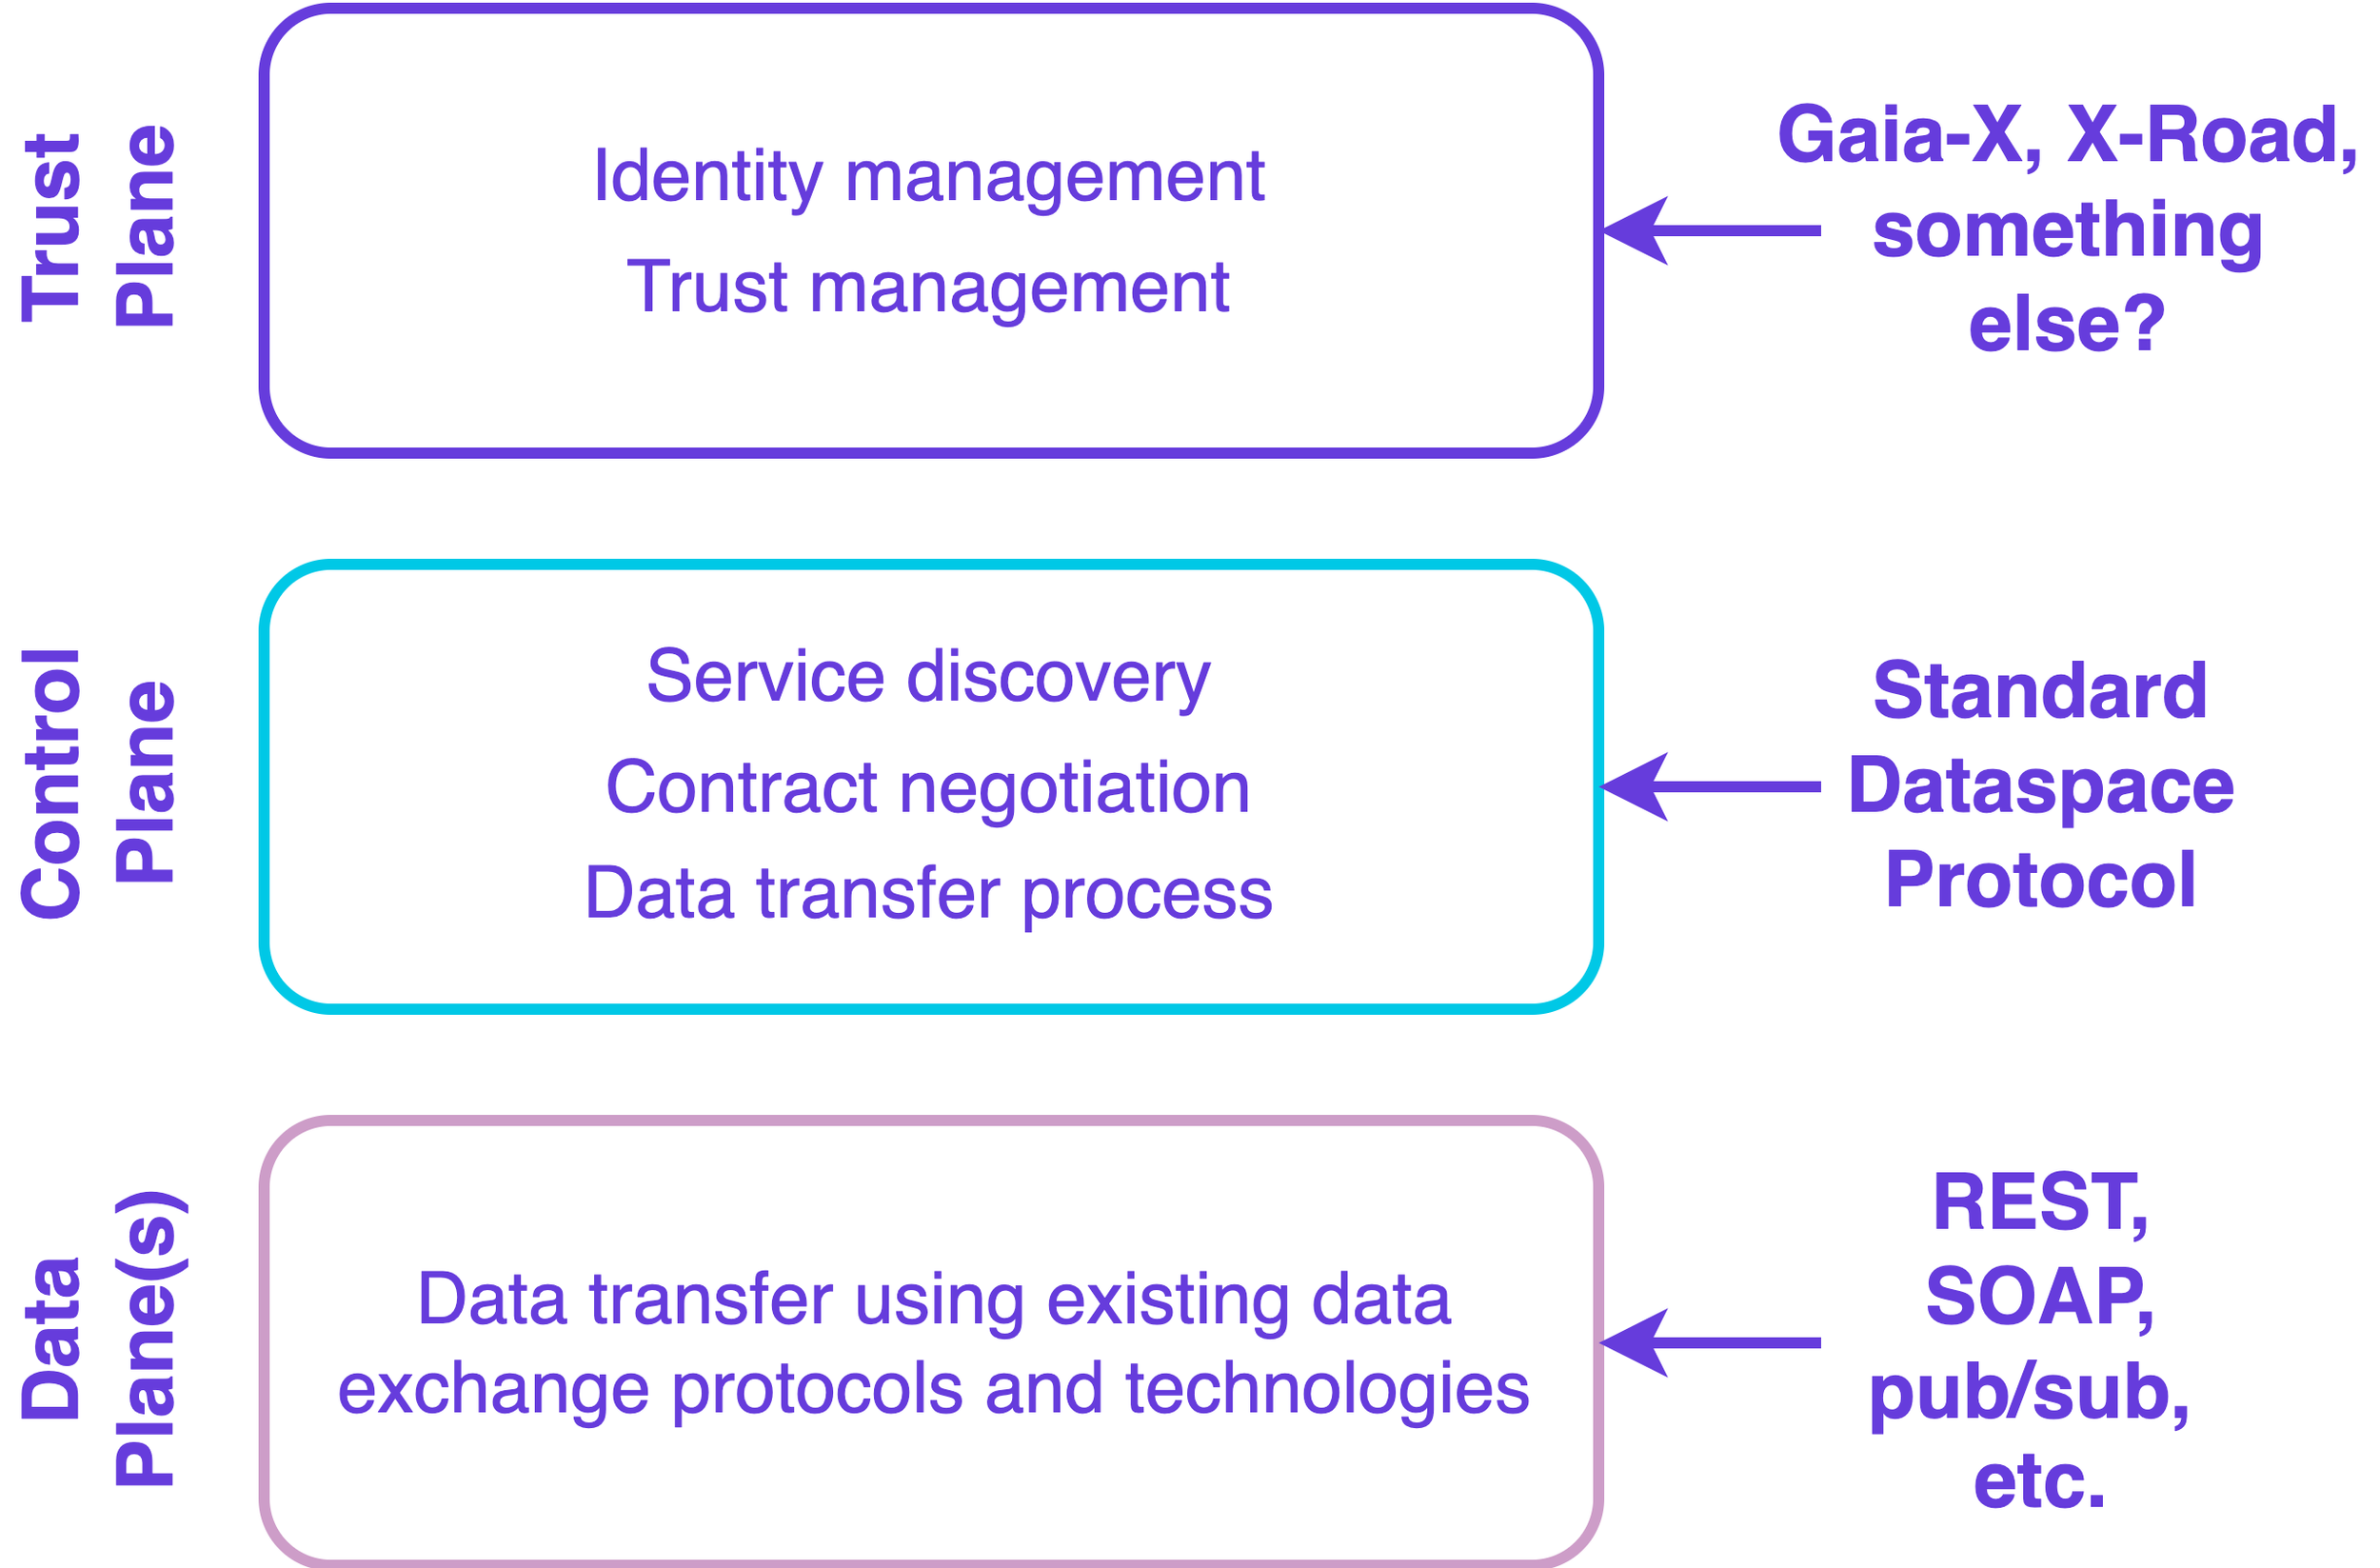
\includegraphics[width=0.6\linewidth]{figures/dataspace_protocol_layers.png}
    \caption[The three-plane dataspace stack]{The three-plane dataspace stack: a Trust Plane for identity and trust, a Control Plane standardised by the Dataspace Protocol, and one or more Data Planes that carry the actual bytes using existing exchange protocols. Figure adapted from~\citep{niisXRoadDataspaceStack}.}
    \label{fig:dsp-planes}
\end{figure}

Within this Control-Plane scope the specification has matured through two governance phases. DSP started under IDSA stewardship and reached its 2024-1 release in that setting; governance has since transferred to the Eclipse Dataspace Working Group, and the version this thesis tracks is the 2025-1 release maintained as an Eclipse Specification project~\citep{datapsaceProtocol2025}. In December 2025 the Eclipse Foundation announced that the Dataspace Protocol, together with the Decentralized Claims Protocol, would be submitted for international standardisation through the ISO/IEC~JTC~1 Publicly Available Specification (PAS) process~\citep{eclipseDspPasSubmission}. The specification is bound to HTTPS for transport and to JSON-LD for message serialisation; each message type is a JSON-LD document POSTed to a well-known endpoint on a peer connector. The specification itself is organised as four documents: \emph{Catalog}, \emph{Contract Negotiation}, and \emph{Transfer Process} cover the three protocol areas, and a \emph{Common} specification covers cross-cutting concerns such as version declaration and the error model. \Cref{fig:dsp-overview} shows how the three protocol areas compose at runtime: two connectors interact directly for cataloging, contract negotiation, and data transfer, with an Identity Provider sitting outside both and serving identity claims to each. The remainder of this section walks through the three protocol areas in the order they execute at runtime~--~discovery first, then negotiation, then transfer.

\begin{figure}[ht]
    \centering
    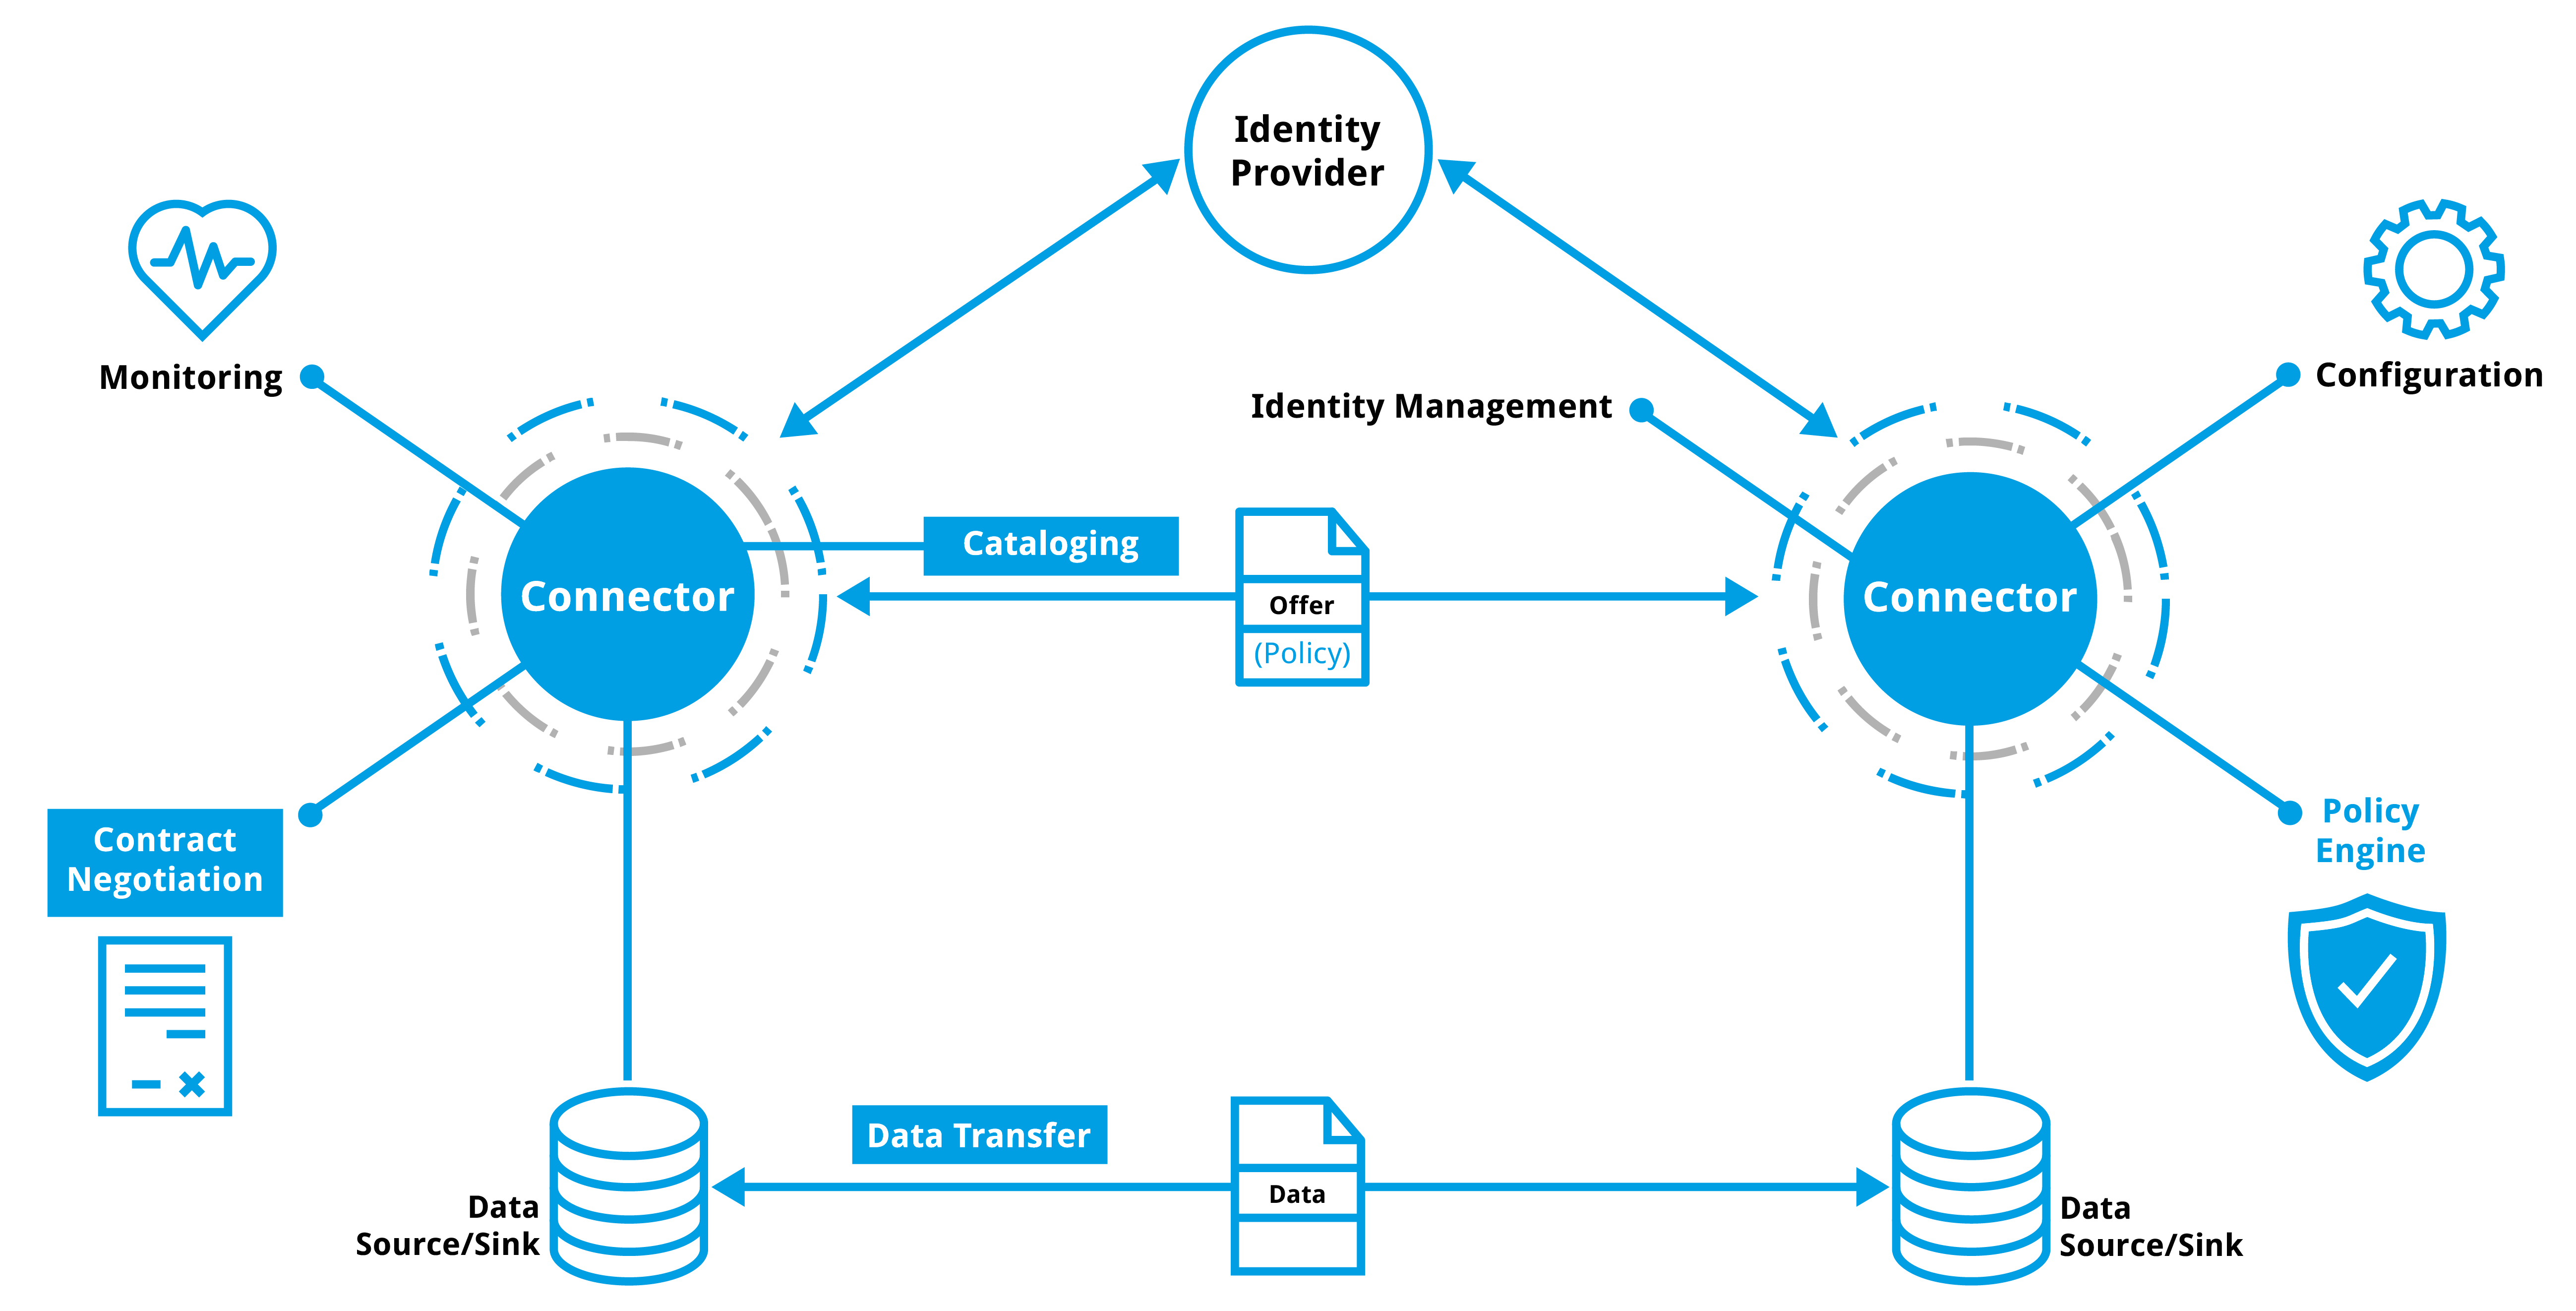
\includegraphics[width=0.85\linewidth]{figures/dsp_protocol_overview.png}
    \caption[Dataspace Protocol overview]{Dataspace Protocol overview: two connectors with an external Identity Provider, exchanging cataloging, contract negotiation, and data-transfer interactions, with policy enforcement and monitoring as cross-cutting concerns on each side. Figure from the Dataspace Protocol specification~\citep{datapsaceProtocol2025}, licensed under Apache~2.0.}
    \label{fig:dsp-overview}
\end{figure}

\paragraph{Catalog Protocol.} The Catalog Protocol governs how a Consumer discovers what Datasets a Provider offers and on what terms. Its data model reuses two existing W3C vocabularies: \emph{DCAT}, the Data Catalog Vocabulary, provides the structure of catalogs and datasets, and \emph{ODRL}, the Open Digital Rights Language, provides the policy expressions that govern subsequent use. A DSP \emph{Catalog} is therefore ``a DCAT Catalog with the following restrictions''~\citep{datapsaceProtocol2025} and carries a \texttt{dspace:participantId} identifying the providing participant. Catalogs contain Datasets; Datasets contain Distributions; each Distribution exposes a DataService whose endpoint URL is where contract negotiation and transfer can later be initiated. ODRL Offers attached to Datasets via the \texttt{hasPolicy} property express the usage policy a Consumer must accept to obtain the data.

Two message types drive the protocol, both sent from Consumer to Provider: the \emph{Catalog Request Message}, which returns the set of Datasets the requester is permitted to see (optionally narrowed by a filter), and the \emph{Dataset Request Message}, which returns a single Dataset by identifier. Both interactions are single round trips, and the Catalog Protocol ``is designed to be used by federated services without the need for a replication protocol''~\citep{datapsaceProtocol2025}: each Consumer issues catalog requests directly to one or more Catalog Services~--~the endpoints that host the Catalog~--~and manages the results locally. Of the three protocols this is the lightest, and the benchmark methodology in \Cref{chap:methodology} accordingly treats catalog requests as a baseline against which the heavier negotiation and transfer flows can be normalised.

\paragraph{Contract Negotiation Protocol.} Once a Consumer has identified a Dataset of interest in the catalog, the Contract Negotiation Protocol establishes a binding ODRL Agreement governing its future use between Provider and Consumer. The protocol is structured as a state machine, reproduced in \Cref{fig:dsp-cn}, with six non-terminal states~--~\textsc{requested}, \textsc{offered}, \textsc{accepted}, \textsc{agreed}, \textsc{verified}, \textsc{finalized}~--~and a single terminal \textsc{terminated} state reachable from any non-terminal state by either party~\citep{datapsaceProtocol2025}. Six message types drive the transitions; the happy path is best read in two halves.

The first half exchanges an offer. The Consumer opens the negotiation with a \emph{Contract Request Message}, placing it in \textsc{requested}; the Provider responds with a \emph{Contract Offer Message} and the negotiation moves to \textsc{offered}; the Consumer signals its acceptance via a \emph{Contract Negotiation Event Message} (with payload \texttt{accepted}), moving it to \textsc{accepted}. The second half seals the agreement. The Provider issues a \emph{Contract Agreement Message} carrying the binding ODRL Agreement and the negotiation moves to \textsc{agreed}; the Consumer acknowledges with a \emph{Contract Agreement Verification Message}, moving it to \textsc{verified}; and the Provider closes the loop with a second \emph{Contract Negotiation Event Message} (with payload \texttt{finalized}), placing the negotiation in \textsc{finalized}~\citep{datapsaceProtocol2025}. At any point either party may send a \emph{Contract Negotiation Termination Message} to abort the sequence.

\begin{figure}[ht]
    \centering
    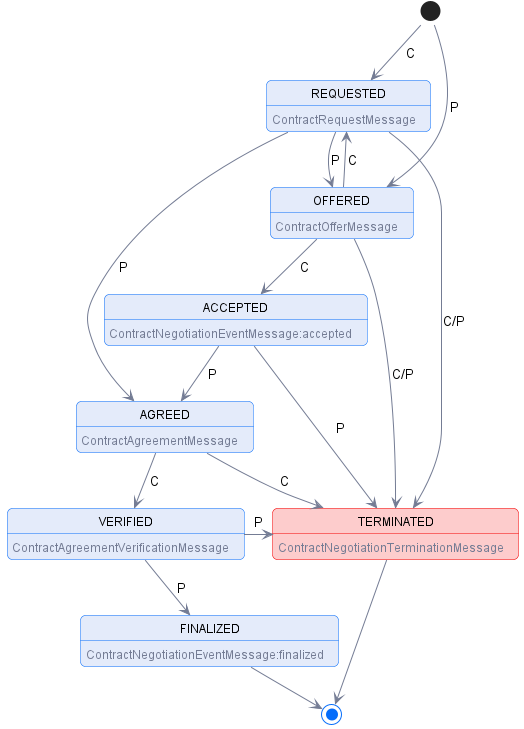
\includegraphics[width=0.6\linewidth]{figures/dsp_cn_state_machine.png}
    \caption[Contract Negotiation state machine in DSP 2025-1]{Contract Negotiation state machine in DSP 2025-1. Transitions labelled \texttt{C} are sent by the Consumer, \texttt{P} by the Provider, and \texttt{C/P} by either. The terminal state \textsc{terminated} is reachable from every non-terminal state. Figure from the Dataspace Protocol specification~\citep{datapsaceProtocol2025}, licensed under Apache~2.0.}
    \label{fig:dsp-cn}
\end{figure}

The negotiation is therefore an inherently asynchronous, multi-message workflow rather than a single request/response. In the happy path it generates six stateful HTTPS exchanges, each requiring the receiving connector to (i)~verify the sender's identity against the Trust Plane, (ii)~evaluate the ODRL policy in scope at the current state, and (iii)~persist the resulting state transition before acknowledging. This is the asynchronous control-plane workflow that classical synchronous-API benchmarking instruments are not designed to measure; \Cref{sec:benchmarking-fundamentals} returns to the methodological consequences.

\paragraph{Transfer Process Protocol.} Once an Agreement is in place, the Consumer may initiate one or more \emph{Transfer Processes} against it. The Transfer Process Protocol governs the lifecycle of each such process through a smaller state machine~--~\textsc{requested}, \textsc{started}, optionally \textsc{suspended}, and the terminal states \textsc{completed} and \textsc{terminated}~--~reproduced in \Cref{fig:dsp-tp}~\citep{datapsaceProtocol2025}. Five message types drive the transitions; three carry the happy path and two handle interruptions.

The happy path is short. The Consumer opens the process with a \emph{Transfer Request Message}, placing it in \textsc{requested}; the Provider responds with a \emph{Transfer Start Message} and the process moves to \textsc{started}; and either party closes it cleanly with a \emph{Transfer Completion Message}, placing it in the terminal \textsc{completed} state. Outside the happy path, either party may send a \emph{Transfer Suspension Message} to pause the process in \textsc{suspended} (from which it can return to \textsc{started}) or a \emph{Transfer Termination Message} to abort it in \textsc{terminated}~\citep{datapsaceProtocol2025}.

\begin{figure}[ht]
    \centering
    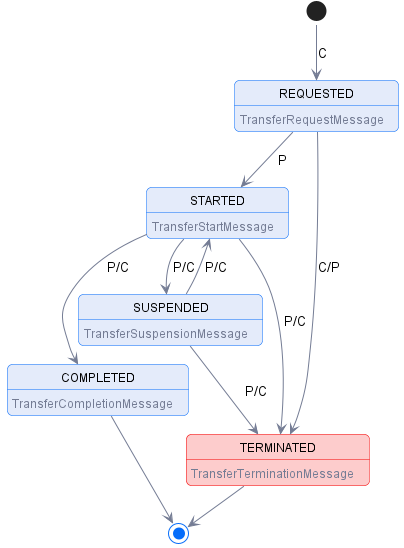
\includegraphics[width=0.5\linewidth]{figures/dsp_tp_state_machine.png}
    \caption[Transfer Process state machine in DSP 2025-1]{Transfer Process state machine in DSP 2025-1. \textsc{completed} and \textsc{terminated} are terminal; \textsc{suspended} may return to \textsc{started}. Figure from the Dataspace Protocol specification~\citep{datapsaceProtocol2025}, licensed under Apache~2.0.}
    \label{fig:dsp-tp}
\end{figure}

The Transfer Process Protocol is also where the control-plane / data-plane separation introduced at the start of this section becomes operational. The specification is explicit: ``services on the control plane receive messages and manage the local state of the TP'' while ``on the data plane, the actual transfer of data takes place using a wire protocol'' whose ``interfaces and interaction patterns are not in scope of this document''~\citep{datapsaceProtocol2025}. Two transfer modes are supported. In a \emph{push} transfer the Consumer includes its own endpoint in the Transfer Request as a \texttt{dataAddress}, and the Provider's data plane pushes bytes to that address as soon as the process enters \textsc{started}. In a \emph{pull} transfer the Provider includes its endpoint in the Transfer Start Message, and the Consumer's data plane pulls bytes from that address. In both modes the \texttt{dataAddress} carries an opaque \texttt{authorization} token whose \texttt{authType} (for example, \texttt{bearer}) tells the receiving side how to present it~\citep{datapsaceProtocol2025}. The control-plane traffic in the happy path is fixed at three messages~--~\textsc{request}, \textsc{start}, \textsc{completion}~--~regardless of payload size, while the data-plane time scales with payload size and the chosen wire protocol. Below some crossover payload size the connector is therefore control-plane bound and above it data-plane bound, an observation that motivates the throughput experiments designed in \Cref{chap:methodology} and the payload-size sweeps reported in \Cref{chap:results-evaluation}.

\paragraph{End-to-end accounting.} A single Provider-to-Consumer exchange in DSP comprises one catalog request, six contract-negotiation messages in the happy path, three transfer-process messages, and an arbitrary number of bytes on the data plane. All four implementations evaluated in \Cref{sec:connectors} conform to the same state machines and the same message schemas, but they differ in how aggressively they pipeline these exchanges, how negotiation and transfer state is persisted between messages, and how the data plane is bridged into and out of the connector. These are the system-layer choices the IDS-RAM placed deliberately outside the specification~\citep{IDS4.0}, and they are the choices whose performance consequences this thesis sets out to measure.

\newpage

\section{Dataspace Connectors}\label{sec:connectors}

The Dataspace Protocol specified in \Cref{sec:dsp} defines what two connectors say to each other; this section describes the runtimes that say it. A \emph{dataspace connector} is the software agent the IDS Reference Architecture places at its System Layer~\citep{IDS4.0}: it carries the connector's catalog, evaluates the policy on every interaction, drives the contract-negotiation and transfer-process state machines defined in \Cref{sec:dsp}, and bridges the dataspace into and out of the participant's own data sources. \Cref{fig:ids-ram-system-components} shows the connector's standard runtime environment as defined by the IDS-RAM: a Provider connector and a Consumer connector at the centre of an ecosystem that also includes a Metadata Broker, a Clearing House, an App Store, and a Vocabulary Hub. The remainder of this section first introduces the Eclipse Dataspace Components (EDC) project~--~the open-source framework that has become the de-facto reference implementation of this connector role~--~and then profiles the four EDC-based and EDC-adjacent implementations whose performance this thesis benchmarks.

\begin{figure}[ht]
    \centering
    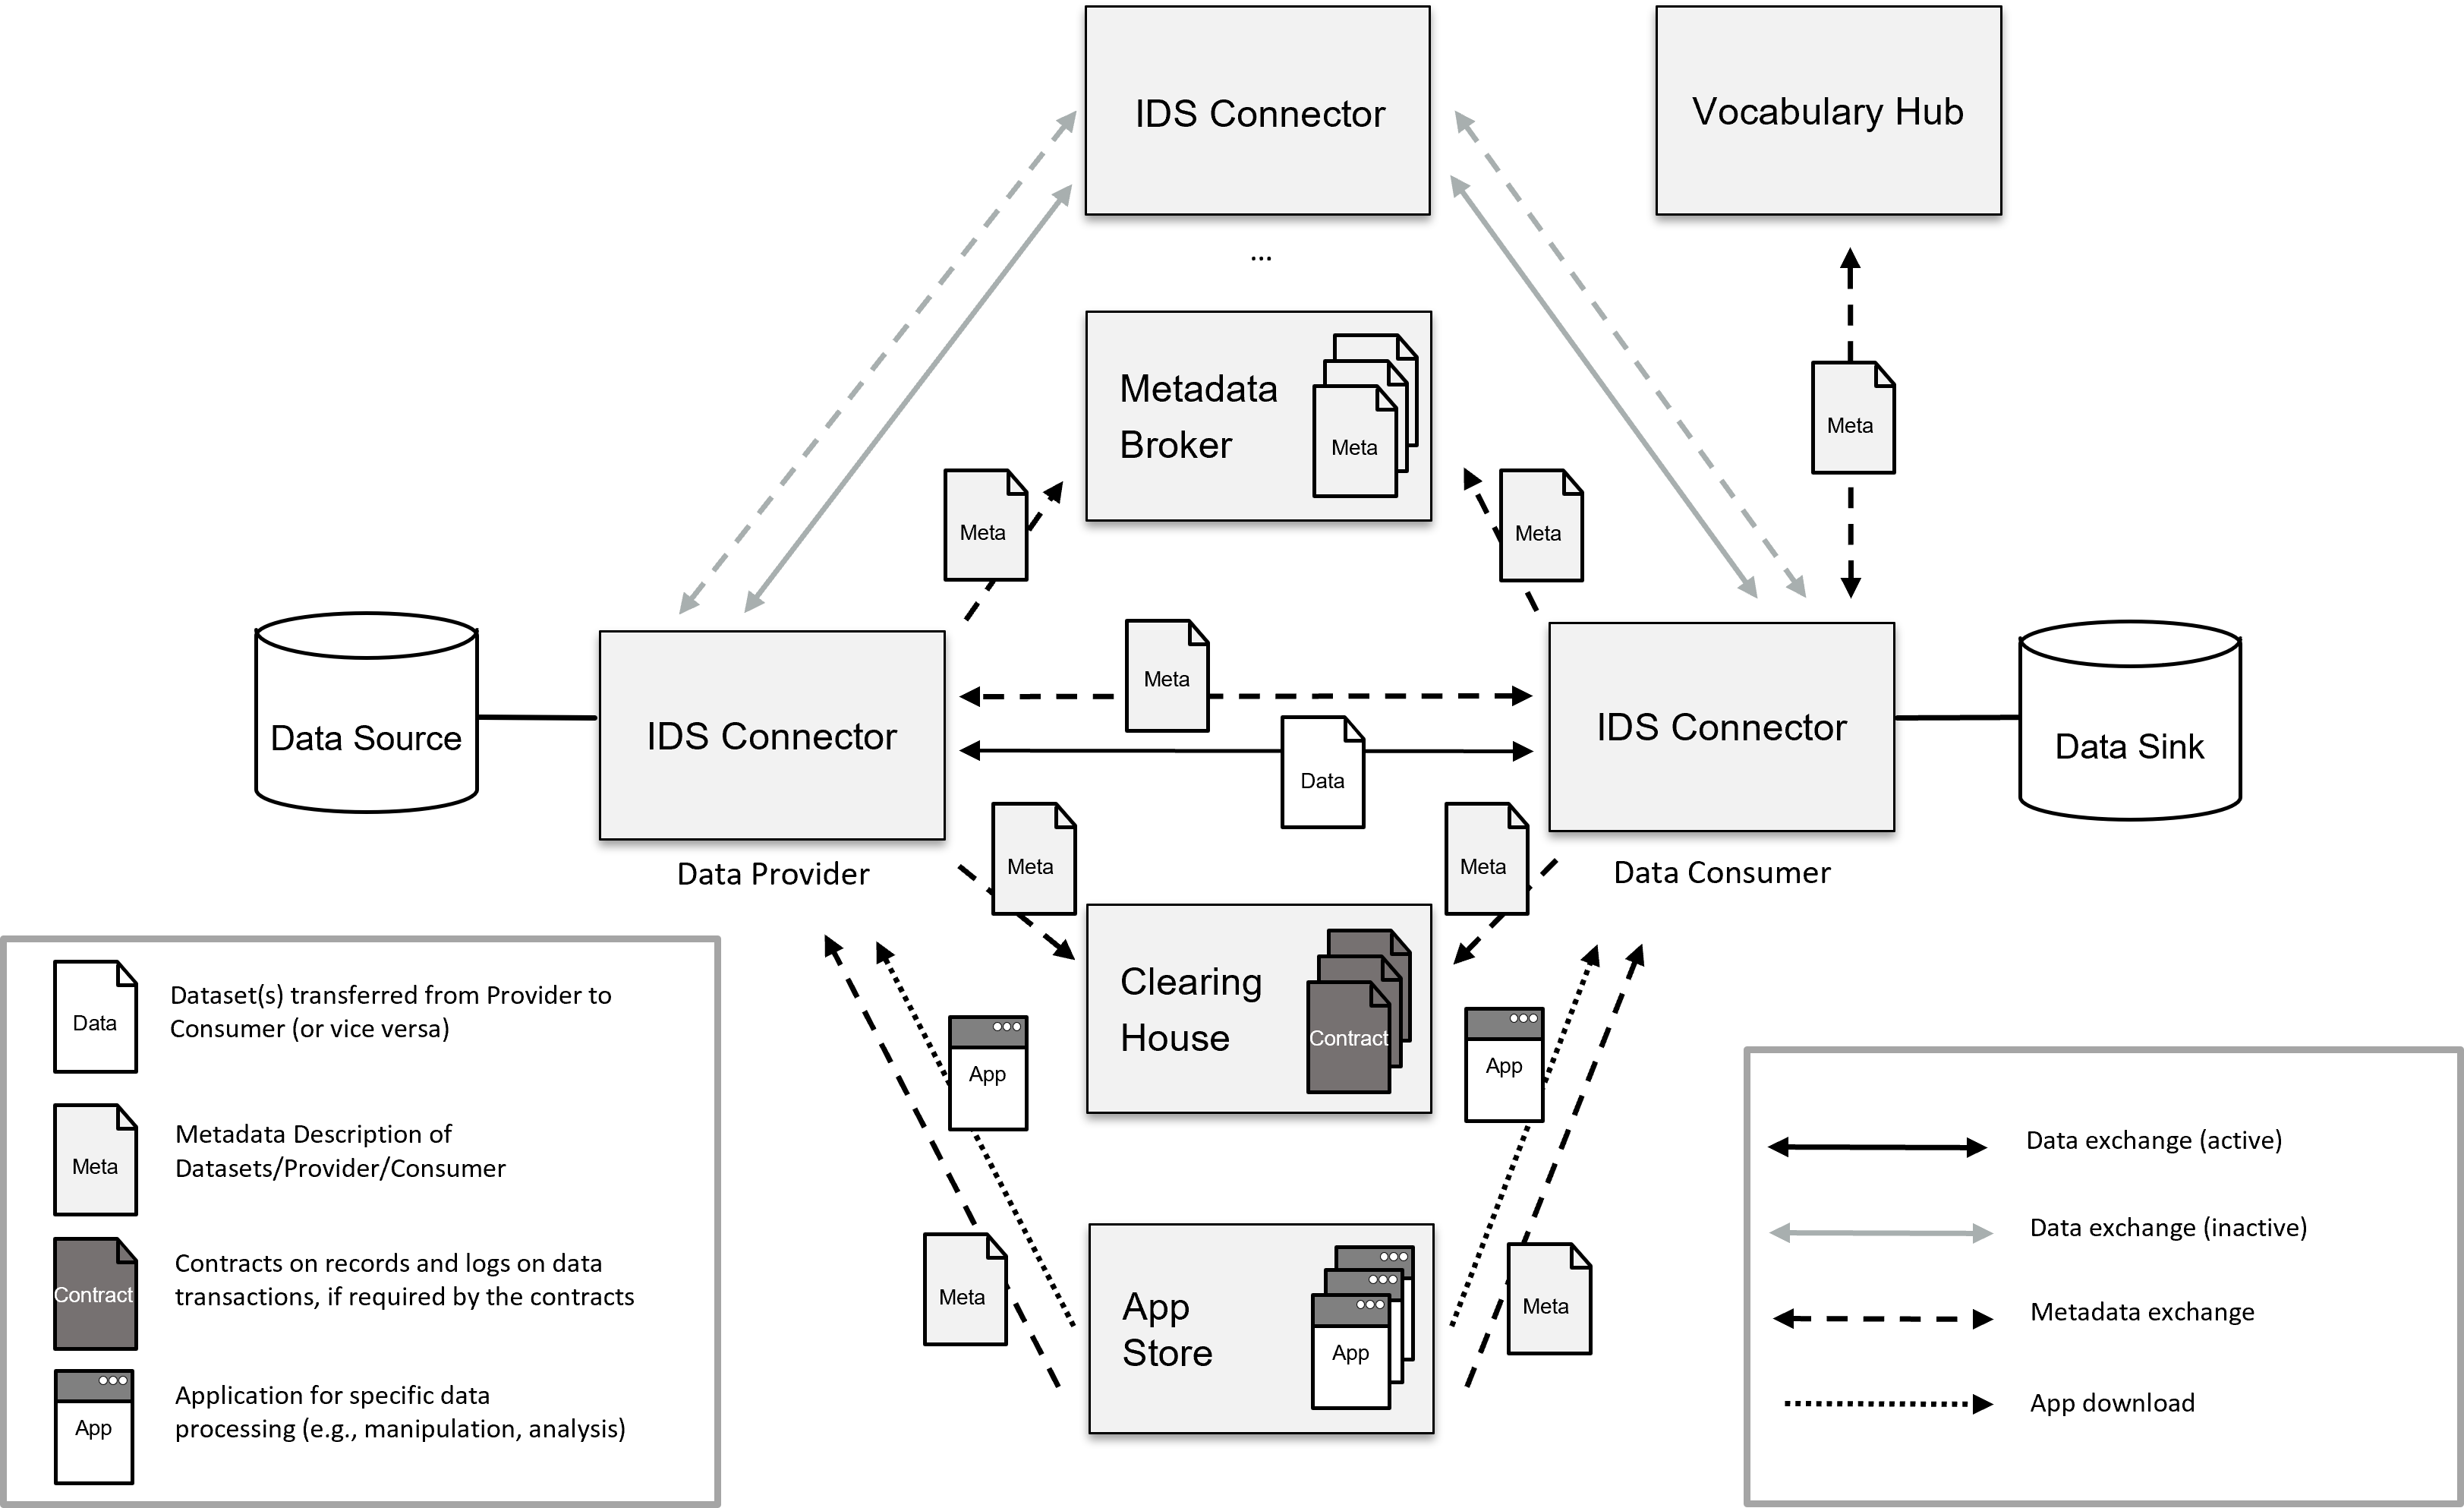
\includegraphics[width=0.85\linewidth]{figures/ids_ram_system_components.png}
    \caption[Standard runtime environment of a dataspace connector]{Standard runtime environment of a dataspace connector as defined by the IDS-RAM: a Data Provider connector and a Data Consumer connector at the centre, surrounded by the Metadata Broker, Clearing House, App Store, and Vocabulary Hub intermediaries. Figure from the IDS-RAM~4 documentation~\citep{IDS4.0}, licensed under CC BY~4.0.}
    \label{fig:ids-ram-system-components}
\end{figure}


\subsection{Eclipse Dataspace Components (EDC)}\label{subsec:edc}

The \emph{Eclipse Dataspace Components} (EDC) project is the open-source framework that has become the de-facto reference implementation of the dataspace connector role described above~\citep{eclipseEdcProject, dam2024surveydataspaceconnectorimplementations}. EDC is governed by the \emph{Eclipse Dataspace Working Group}, launched in December~2023 under the Eclipse Foundation AISBL with founding members including Amadeus, Fraunhofer, IDSA, iSHARE, Microsoft, and T-Systems~\citep{eclipseDswg}. The project itself sits in the Eclipse Technology top-level project and is released under the Apache~2.0 licence~\citep{eclipseEdcProject}. EDC implements the IDS Reference Architecture Model and the Dataspace Protocol introduced in \Cref{sec:data-spaces-ids,sec:dsp}, and is the source from which three of the four implementations evaluated in \Cref{subsec:different-connectors} are derived~\citep{eclipseEdcDocumentation, dam2024surveydataspaceconnectorimplementations}.

Architecturally, EDC realises the abstract IDS connector~--~shown in \Cref{fig:ids-ram-connector-functional} as the IDS-RAM specifies it~--~as three loosely coupled subsystems~\citep{eclipseEdcDocumentation, IDS4.0}:

\begin{description}
    \item[Control Plane.] Owns the state machines of \Cref{sec:dsp}: it handles catalog requests, drives contract negotiation, evaluates usage policies, and coordinates each transfer process from initiation to its terminal state.
    \item[Data Plane.] Carries out the corresponding data-plane work~--~actual byte movement over the wire protocol chosen by the deployment (HTTP push or pull, S3-style object stores, Kafka, and others)~--~and is deliberately separated from the Control Plane so that a long transfer cannot stall the negotiation of another.
    \item[Management API.] A REST interface through which operators and integrating applications create and observe Assets, Policies, Contract Definitions, and Transfer Processes; all mutations through this API are asynchronous, so the Control Plane's own state machines remain authoritative.
\end{description}

The codebase is correspondingly partitioned into four modules~\citep{eclipseEdcDocumentation}:

\begin{itemize}
    \item the \emph{Service Provider Interface (SPI)} module, which defines the extension points;
    \item the \emph{Core} module, which provides the default state-machine and policy engines;
    \item a set of \emph{Extensions} for specific technologies (databases, object stores, vaults);
    \item the \emph{Data Protocols} module, which contains the DSP binding itself.
\end{itemize}

\begin{figure}[ht]
    \centering
    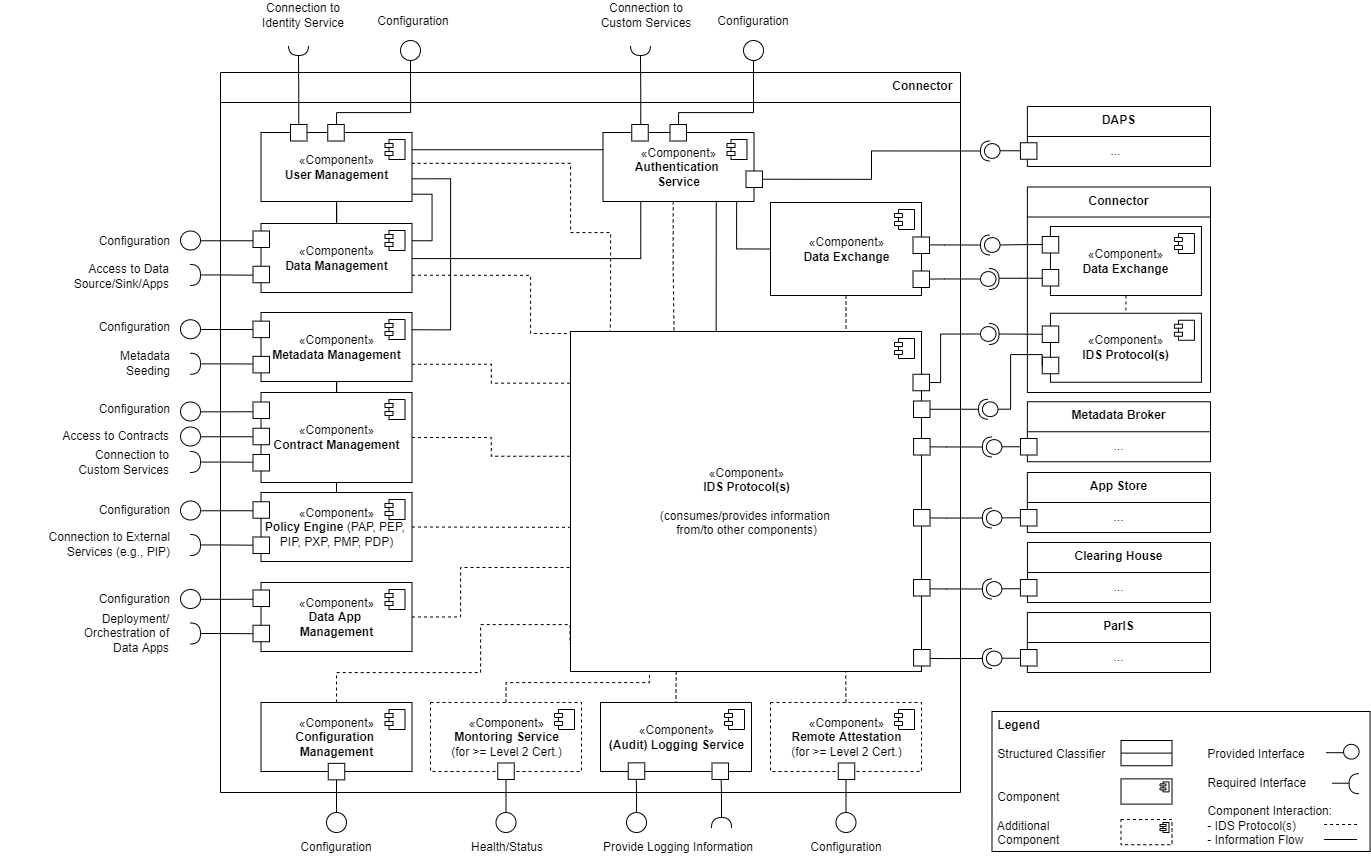
\includegraphics[width=0.95\linewidth]{figures/ids_ram_connector_functional_view.png}
    \caption[Functional view of an IDS connector]{Functional view of an IDS connector as defined by the IDS-RAM: internal components for User Management, Authentication, Data, Metadata, Contract, Policy, and App Management, the IDS Protocol engine, and external interfaces to the Identity Service (DAPS), Metadata Broker, App Store, Clearing House, and Participant Information Service (ParIS). EDC instantiates this functional surface as the modular Control Plane / Data Plane / Management API architecture described in the surrounding paragraphs. Figure from the IDS-RAM~4 documentation~\citep{IDS4.0}, licensed under CC BY~4.0.}
    \label{fig:ids-ram-connector-functional}
\end{figure}

The composition of an EDC runtime is determined entirely by the set of \emph{ServiceExtensions} loaded at startup~\citep{eclipseEdcDocumentation}. Every feature of a running connector~--~persistence backend, identity provider, data-plane transport, policy evaluator, telemetry sink~--~is contributed by an extension that implements the \texttt{ServiceExtension} interface and declares its dependencies through the \texttt{@Inject} annotation. The runtime resolves these declarations and drives all extensions through a five-phase lifecycle: \texttt{inject}, \texttt{initialize}, \texttt{provide}, \texttt{prepare}, \texttt{start}~\citep{eclipseEdcDocumentation}. This architectural choice has one direct consequence for the present thesis: an EDC distribution is not a single binary but a curated bundle of extensions, and most of the variation across the implementations profiled in \Cref{subsec:different-connectors} lives in \emph{which} extensions each variant bundles and \emph{which} EDC core version they bundle against.

For the Trust Plane introduced in \Cref{sec:dsp}, EDC has moved away from the original IDS-era \emph{Dynamic Attribute Provisioning Service} (DAPS), which the project now explicitly discourages on the grounds of its centralised trust anchor~\citep{eclipseEdcDocumentation}. The currently recommended identity layer is the \emph{Decentralized Claims Protocol} (DCP), a specification carried forward by the Eclipse DSWG as ``an interoperable overlay to the Dataspace Protocol (DSP) Specifications for conveying organizational identities and establishing trust in a way that preserves privacy and limits the possibility of network disruption''~\citep{dcpSpec}. DCP relies on W3C Decentralized Identifiers and Verifiable Credentials and is realised by two concrete wallet components evaluated in \Cref{subsec:different-connectors}: the \emph{EDC IdentityHub}, an EDC-native DCP wallet implementation~\citep{eclipseEdcIdentityHub}, and the \emph{Decentralized Identity Management} (DIM) service used by the Tractus-X profile.

Persistence in EDC is also an extension choice rather than a fixed runtime feature~\citep{eclipseEdcDocumentation}. The default development runtime uses in-memory stores for Assets, Contract Negotiations, and Transfer Processes; production deployments typically replace these with the SQL extension backed by PostgreSQL and pair it with HashiCorp Vault for secret material. Three of the four implementations evaluated in \Cref{subsec:different-connectors} adopt exactly this PostgreSQL + Vault combination; the fourth replaces the entire EDC persistence layer with a MongoDB-backed alternative library, a divergence the next subsection returns to.

These three architectural choices~--~the Control Plane / Data Plane / Management API split, the ServiceExtension composition model, and the pluggable identity and persistence layers~--~together explain why a single Eclipse project has spawned a heterogeneous family of downstream connectors rather than a single canonical distribution. The next subsection profiles the four members of that family that this thesis benchmarks.


\subsection{Different Connector Implementations}\label{subsec:different-connectors}

Four DSP-conformant implementations are in scope for the benchmarks reported in \Cref{chap:results-evaluation}: \emph{Tractus-X EDC}, \emph{Factory-X EDC}, \emph{DSP-Native BaSyx}, and the \emph{Fraunhofer ISST EDC}. Three of the four are EDC distributions in the sense of \Cref{subsec:edc}~--~bundles of EDC core plus chosen extensions~--~and the fourth is an architectural outlier built on a different framework entirely. The four differ along four axes that recur in the comparison: (a) the EDC core version they track, where applicable; (b) the identity stack they integrate; (c) the persistence and deployment topology they ship; and (d) the consortium and use case they target. \Cref{tab:connector-comparison} at the end of this subsection summarises the result. Existing cross-implementation surveys cover features and protocol compliance but explicitly defer performance evaluation~\citep{dam2024surveydataspaceconnectorimplementations}; the per-connector profiles below provide the architectural background against which the measured differences in \Cref{chap:results-evaluation} can be interpreted.

\paragraph{Tractus-X EDC.} The \emph{Tractus-X EDC} is the official connector distribution for the Catena-X automotive dataspace, maintained inside the Eclipse Tractus-X project of the Eclipse Foundation~\citep{tractusxEdc}. The repository describes itself as the source of ``Container images and deployments of the Eclipse Dataspace Components for the Tractus-X project''~\citep{tractusxEdc} and ships two production-ready runtime distributions: \texttt{edc-controlplane-postgresql-hashicorp-vault} and \texttt{edc-dataplane-hashicorp-vault}, both pinned in the benchmarked configuration to EDC core version~0.15.1. The identity stack is DCP backed by the Catena-X \emph{Decentralized Identity Management} (DIM) service, with a dedicated Secure Token Service extension that mediates between the connector and DIM. Beyond vanilla EDC, Tractus-X bundles extensions specific to the Catena-X governance model: Business Partner Number (BPN) validation, a federated catalog with connector discovery via a Business Discovery and Registration Service client, the v2 Endpoint Data Reference API with callback support, and Catena-X-specific contract-policy validation. Its target dataspace is the supplier-to-OEM data exchange of Catena-X~\citep{catenaxDocumentation, tractusxEdc}.

\paragraph{Factory-X EDC.} The \emph{Factory-X EDC} is a downstream profile of Tractus-X EDC adapted for the discrete-manufacturing dataspace operated by the Factory-X consortium~\citep{factoryxEdc, factoryxConsortium}. The Factory-X consortium itself is co-chaired by Siemens and SAP with roughly fifty additional commercial and research partners, and the EDC repository is explicit about its proof-of-concept status: ``Factory-X has not yet agreed on any normative specifications, an operating model, an identity stack or a security architecture. This repository is a contribution to that conversation demonstrating the feasibility of the Dataspace Protocol and the Decentralized Claims Protocol as common protocol foundation''~\citep{factoryxEdc}. The benchmarked configuration pins EDC core version~0.14.0~--~one minor version behind Tractus-X~--~and differs from the Tractus-X profile in three load-bearing places. First, it replaces the upstream JSON-LD and Dataspace Protocol modules with Factory-X-specific implementations. Second, it adds a custom \gls{mqtt} transport for the Data Plane alongside the standard HTTP transports. Third, it terminates Data Plane traffic over mutual TLS rather than the more common bearer-token authorisation introduced in \Cref{sec:dsp}. Its identity stack is DCP with custom DID validation rather than the DIM service used by Tractus-X.

\paragraph{DSP-Native BaSyx.} The \emph{DSP-Native BaSyx} connector is the architectural outlier in the comparison: it is not an EDC distribution. The repository describes it as ``a DSP-native variant of the Eclipse BaSyx Asset Administration Shell (AAS) system, built on the Spring Boot framework. It integrates the Dataspace Protocol (DSP) library along with selected components from the Eclipse BaSyx framework''~\citep{dspNativeBasyx}.\glsadd{aas} Architecturally, this means the runtime is a Spring Boot application that embeds Eclipse BaSyx~2.0.0~\citep{eclipseBasyxDocs} for Asset Administration Shell representation and the separate \texttt{dataspace-protocol-lib} library~\citep{dspProtocolLib} (in its MongoDB-backed variant) for the DSP message exchange itself, replacing the entire EDC runtime stack described in \Cref{subsec:edc}. Persistence is MongoDB rather than PostgreSQL, identity in the benchmarked development stack is a Keycloak-issued \gls{jwt} rather than a DCP credential, and asynchronous events use an embedded Eclipse Mosquitto \gls{mqtt} broker. The counterparty in the bundled deployment is itself an EDC connector (Factory-X EDC), which makes the DSP-Native BaSyx versus EDC comparison directly observable inside a single docker-compose stand-up. Its target use case is exposing Industry~4.0 asset descriptions natively over DSP.

\paragraph{Fraunhofer ISST EDC.} The \emph{Fraunhofer ISST EDC} is the EDC extensions and runtime distribution maintained by the Dataspace Technologies (DST) department of Fraunhofer ISST~\citep{fraunhoferIsstDst}. The repository describes itself as the source of ``all EDC extensions and runtimes from the DST department'', with a uniform semantic version of the form \texttt{<DST-Version>-<EDC-Version>} that records both its own iteration and the EDC core baseline against which the extensions are built; the benchmarked configuration tracks EDC core version~0.15.1. Its distinguishing architectural choice is the depth of its identity integration. Where Tractus-X integrates DCP at the connector boundary and Factory-X integrates DCP plus a custom DID validator, the Fraunhofer ISST distribution bundles the full EDC identity stack as separate runtimes alongside the connector itself: an \texttt{identity-hub-persistence} runtime instantiating the EDC IdentityHub~\citep{eclipseEdcIdentityHub} and an \texttt{issuer-service-persistence} runtime that issues the verifiable credentials the IdentityHub then presents. DCP is wired through all three EDC subsystems~--~Control Plane, Data Plane, and Federated Catalog~--~rather than only at the connector boundary. This distribution should not be confused with the unrelated and now-archived \texttt{FraunhoferISST/DataspaceConnector} project of 2022, which was an IDS-native connector that predates the Dataspace Protocol and is not part of this thesis.

\clearpage

\begin{table}[ht]
    \centering
    \caption[Architectural profile of the four connector implementations]{Architectural profile of the four connector implementations evaluated in this thesis.}
    \label{tab:connector-comparison}
    \small
    \setlength{\tabcolsep}{4pt}
    \begin{tabularx}{\textwidth}{@{}l l X X X@{}}
        \toprule
        \textbf{Connector} & \textbf{EDC core} & \textbf{Identity stack} & \textbf{Persistence} & \textbf{Distinctive feature} \\
        \midrule
        Tractus-X EDC       & 0.15.1      & DCP + DIM            & PostgreSQL + Vault & BPN validation, federated catalog    \\
        Factory-X EDC       & 0.14.0      & DCP + DID validation & PostgreSQL + Vault & \gls{mqtt} transport, mTLS data plane      \\
        DSP-Native BaSyx    & n/a (BaSyx) & Keycloak (dev)       & MongoDB            & AAS-native, non-EDC                  \\
        Fraunhofer ISST EDC & 0.15.1      & DCP + IdentityHub    & PostgreSQL + Vault & Bundled IdentityHub + Issuer Service \\
        \bottomrule
    \end{tabularx}
\end{table}

The architectural diversity tabulated above is precisely why \Cref{chap:related-work} can identify only one prior cross-implementation performance study~\citep{evaluatingtheperformanceimpactofdatasovereignty}: the test surface is large and the implementations make non-trivially different design choices. \Cref{chap:methodology} defines the workload that exercises these four implementations under comparable conditions, \Cref{chap:implementation} describes the deployed configuration in full, and \Cref{chap:results-evaluation} reports the measured consequences of the architectural differences summarised here.


\section{Performance Concepts}\label{sec:performance-concepts}

Comparing the four implementations of \Cref{sec:connectors} requires performance to be defined in measurable terms rather than left as an intuition. This thesis adopts the vocabulary of ISO/IEC~25010, which models \emph{performance efficiency} through three sub-characteristics: \emph{time behaviour} (the response times and throughput a system achieves under stated conditions), \emph{resource utilisation} (the amounts and types of resources it consumes), and \emph{capacity} (the maximum limits it can sustain)~\citep{iso25010}. The two subsections that follow map onto this division: \Cref{subsec:performance-metrics} treats time behaviour and capacity~--~latency, throughput, and how both scale with load~--~and \Cref{subsec:resource-util} treats resource utilisation. Each concept is defined here against its primary source and paired with the concrete signal that the thesis instruments for it; the full measurement pipeline (OpenTelemetry to Prometheus to Grafana) is described in \Cref{chap:implementation}, and the measured values are reported in \Cref{chap:results-evaluation}.


\subsection{Throughput, Latency, and Scalability}\label{subsec:performance-metrics}

\paragraph{Latency.} The latency, or response time, of a request is the interval between its submission and the completion of its response. In queueing terms, this interval decomposes into \emph{waiting time}~--~spent in a queue before processing begins~--~and \emph{service time}~--~spent in actual processing~\citep{jain1991art}; the distinction matters because, as later paragraphs show, the two respond differently to load. A single latency figure is rarely sufficient. For request--response systems the user-relevant quantity is the \emph{distribution} of response times, and in particular its tail: in large-scale services, rare slow responses dominate the user-perceived experience, and the recurring causes of latency variability are ``queueing'', shared-resource contention, ``maintenance activities'', and ``periodic garbage collection in garbage-collected languages''~\citep{dean2013tail}. Two consequences follow for this thesis. First, latency is reported not as a mean but as the median and the 95th and 99th percentiles, computed from the request-duration histogram exposed by each connector (\cref{subsec:resource-util} returns to the garbage-collection cause, which is directly observable in the same deployment). Second, a complete \gls{dsp} exchange is not a single request but the asynchronous, multi-message negotiation-and-transfer cycle of \Cref{sec:dsp}; its end-to-end latency is the sum of the per-message latencies across two state machines, and is reconstructed from distributed traces that span both the provider-side and consumer-side runtimes. This end-to-end view is the one that bears on the asynchronous-cycle research question of \Cref{chap:introduction}.

\paragraph{Throughput.} Throughput is the rate at which a system completes work, expressed for the present purpose in requests or completed transfers per unit time~\citep{jain1991art}. Throughput does not rise without bound as offered load increases: every system has a \emph{capacity}, and as load approaches it the system passes through a \emph{knee} beyond which throughput plateaus while latency climbs steeply, a regime characterised as saturation~\citep{jain1991art}. \Cref{fig:knee-curve} sketches this relationship. Throughput, latency, and the number of concurrent requests in the system are not independent: Little's Law states that for a stable system the mean number of requests in residence equals the product of the arrival rate and the mean response time, $L = \lambda W$~\citep{little1961proof}, a relation this thesis uses to cross-check that measured throughput, concurrency, and latency are mutually consistent. Throughput is instrumented as the rate of completed requests per endpoint, separated by connector runtime so that the provider and consumer sides can be attributed independently.

\begin{figure}[ht]
    \centering
    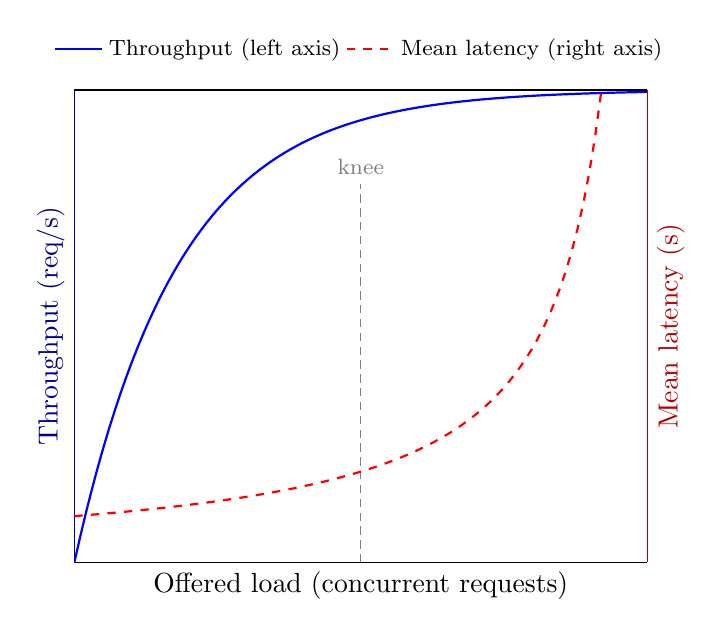
\begin{tikzpicture}
        % 'scale only axis' forces both axes to share the EXACT same plot
        % rectangle, so the right-hand y-axis and its label line up on the
        % right instead of overlapping the plot.
        % Left axis: throughput (solid, blue) -- label coloured to match curve.
        \begin{axis}[
            scale only axis,
            width=0.6\linewidth, height=6cm,
            xlabel={Offered load (concurrent requests)},
            axis y line*=left,
            ylabel={Throughput (req/s)},
            ylabel near ticks,
            ylabel style={text=blue!55!black},
            y axis line style={blue!55!black},
            xtick=\empty, ytick=\empty,
            xmin=0, xmax=10, ymin=0, ymax=10,
            domain=0:10, samples=100,
            every axis plot/.append style={thick},
        ]
            % Throughput: rises ~linearly, then saturates (knee around x=5)
            \addplot[blue]{10*(1-exp(-0.55*x))};
            \label{plot:throughput}
            % saturation/knee marker
            \draw[densely dashed, gray] (axis cs:5,0) -- (axis cs:5,8.0);
            \node[gray, anchor=south, font=\footnotesize] at (axis cs:5,8.0) {knee};
        \end{axis}
        % Right axis: mean latency (dashed, red) -- same plot rectangle.
        \begin{axis}[
            scale only axis,
            width=0.6\linewidth, height=6cm,
            axis y line*=right,
            axis x line=none,
            ylabel={Mean latency (s)},
            ylabel near ticks,
            ylabel style={text=red!70!black},
            y axis line style={red!70!black},
            ytick=\empty,
            xmin=0, xmax=10, ymin=0, ymax=10,
            domain=0:10, samples=100,
            every axis plot/.append style={thick},
            % legend sits ABOVE the plot, so it cannot overlap the curves
            legend style={at={(0.5,1.04)}, anchor=south, legend columns=2,
                          draw=none, fill=none, font=\footnotesize},
            legend cell align=left,
        ]
            % proxy image for the throughput curve (which lives in the other axis)
            \addlegendimage{blue, thick}
            % Latency: flat, then diverges as utilisation -> 1 (knee region)
            \addplot[red, dashed]{1/(1.02-0.1*x)};
            \label{plot:latency}
            \legend{Throughput (left axis), Mean latency (right axis)}
        \end{axis}
    \end{tikzpicture}
    \caption[Throughput and latency versus offered load]{Schematic relationship between throughput (solid, left axis) and mean latency (dashed, right axis) as offered load increases. Throughput rises with load until the system approaches its capacity at the knee, beyond which it plateaus while latency diverges. The shape follows the saturation behaviour of a system approaching its capacity~\citep{jain1991art}; the curves are illustrative, not measured.}
    \label{fig:knee-curve}
\end{figure}

\paragraph{Scalability.} Scalability is the degree to which a system sustains its performance as load or provisioned resources grow. It is achieved either by \emph{vertical} scaling~--~adding resources to a single instance~--~or \emph{horizontal} scaling~--~adding instances~--~and neither is free. Amdahl's law bounds the achievable speed-up by the serial fraction of the work: a computation that is, say, ten per cent inherently sequential cannot be accelerated more than tenfold no matter how many processors are added~\citep{amdahl1967validity}. The Universal Scalability Law generalises this to throughput scaling by adding a \emph{coherency} term for the cost of keeping distributed state consistent; it predicts that throughput first grows sub-linearly, then plateaus, and can even \emph{retrograde} at high concurrency once coherency cost dominates~\citep{gunther2007guerrilla}. A further subtlety concerns how load is generated when scalability is measured. Closed-loop generators, which hold a fixed population of clients each waiting for a response before issuing the next request, can mask the latency degradation that an open arrival model~--~where requests arrive independently of system state~--~would reveal~\citep{schroeder2006open}; the choice between the two materially changes the conclusion, a point \Cref{chap:methodology} returns to when fixing the load model. For this thesis a scalability result is a curve of throughput and tail latency against concurrency, with the per-runtime thread count read as a proxy for the concurrency the connector is actually carrying.


\subsection{Resource Utilisation}\label{subsec:resource-util}

\paragraph{The utilisation--latency relationship.} Resource utilisation is the second sub-characteristic of performance efficiency in ISO/IEC~25010 and covers the degree to which a system consumes processor, memory, storage, and network resources under load~\citep{iso25010}. Utilisation cannot be read in isolation from latency, because the two are coupled through queueing: for a single-server queue the mean response time grows as $W = S/(1-\rho)$, where $S$ is the service time and $\rho$ the utilisation, so that as utilisation approaches unity the response time diverges~\citep{jain1991art}. This is the same divergence that produces the knee in \Cref{fig:knee-curve}, viewed from the resource side rather than the load side, and it is why a connector reporting acceptable latency at moderate utilisation can collapse under a modest further increase in load. Host-level processor and memory utilisation are instrumented through standard operating-system exporters in the deployment described in \Cref{chap:implementation}.

\paragraph{The USE method.} To structure the resource analysis this thesis follows the \gls{use} method, which examines each resource along three axes: \emph{utilisation}, the fraction of time the resource is busy; \emph{saturation}, the degree to which work queues because the resource cannot service it immediately; and \emph{errors}, the count of error events~\citep{gregg2012thinking}. The method's central caution is that high utilisation is not in itself a fault~--~a resource can be busy without a backlog~--~whereas saturation, the accumulation of queued work, is the more reliable indicator of a bottleneck~\citep{gregg2012thinking}. Mapped onto this thesis, utilisation and saturation are observed from host processor, memory, disk, and network metrics, while the errors axis corresponds to the rate of failed (4xx and 5xx) responses recorded per connector runtime.

\paragraph{JVM resources and garbage collection.} Three of the four implementations in \Cref{subsec:different-connectors} run on the Java Virtual Machine, which makes heap occupancy and garbage-collection behaviour first-class resource concerns rather than implementation details. Garbage collection is the concrete instance of the tail-latency cause identified for garbage-collected languages~\citep{dean2013tail}: a stop-the-world pause that coincides with a request inflates that request's response time, so periods of heavy collection appear as spikes in the latency tail. The thesis therefore observes heap usage, the rate of time spent in garbage collection, and the live thread count for each runtime, and reads garbage-collection activity alongside the latency percentiles so that pause-induced tail inflation can be distinguished from genuine processing cost. These quantities are captured as instrument types~--~counters for monotonic counts, gauges for point-in-time levels, and histograms for latency distributions~--~exported under the OpenTelemetry semantic conventions~\citep{opentelemetrySemconv} and stored in Prometheus, whose corresponding metric types define how each series is recorded and queried~\citep{prometheusMetricTypes}. Load is applied with the k6 load generator~\citep{k6docs}. The construction of this pipeline, the load profiles, and the per-connector configuration are the subject of \Cref{chap:methodology,chap:implementation}; the present section has defined only what is measured and why it matters.


\section{Benchmarking Fundamentals}\label{sec:benchmarking-fundamentals}

\Cref{sec:performance-concepts} defined \emph{what} to measure; this section establishes \emph{how} to measure it so that the four implementations of \Cref{sec:connectors} can be compared on equal terms. The instrument for such a comparison is a benchmark.

\paragraph{Benchmarking as systematic performance evaluation.} A benchmark is a standard tool for ``competitively evaluating and comparing'' methods, techniques, or systems with respect to a quality of interest such as performance~\citep{empiricalStandardsBenchmarking}. Benchmarking is therefore not a single measurement but a method: performance evaluation is a systematic procedure in which the analyst first fixes the goal and the system boundary, then selects metrics, workloads, and an evaluation technique, and only then measures~--~each choice made deliberately rather than by default~\citep{jain1991art}. The performance metrics of \Cref{sec:performance-concepts}~--~latency percentiles, throughput, resource utilisation~--~are the first of these choices; the remainder of this section concerns the others and the standards that govern them.

\paragraph{Benchmarking as an empirical standard.} Within software-engineering research, benchmarking has been recognised as a first-class empirical method rather than mere engineering practice~\citep{hasselbring2021benchmarking}. The ACM SIGSOFT \emph{Empirical Standards} codify the expectations for distinct research methods so that studies can be reviewed against method-appropriate criteria rather than a single generic rubric~\citep{Ralph2020}. The initial Empirical Standards lacked a checklist for benchmarking, a gap whose remedy was proposed~\citep{hasselbring2021benchmarking} and now exists as a dedicated benchmarking standard~\citep{empiricalStandardsBenchmarking}. Adopting this standard gives the present work an explicit, externally defined target to satisfy, rather than an ad-hoc notion of a ``fair'' comparison.

\paragraph{What makes a benchmark sound.} The benchmarking standard enumerates the attributes a defensible benchmarking study must exhibit~\citep{empiricalStandardsBenchmarking}. The benchmark itself must be justified~--~either an established, publicly available benchmark is reused or a new one is defined with its measured quality, metrics, measurement method, and workload specified and motivated by relevance. The experimental setup and the workload must each be documented ``in sufficient detail to support independent replication''~\citep{empiricalStandardsBenchmarking}. The compared systems must ``compete on their merits without artificial limitations''~\citep{empiricalStandardsBenchmarking}~--~the fairness condition that is the central difficulty when the systems differ architecturally, as the four connectors of \Cref{subsec:different-connectors} do. Finally, the study must assess stability ``using sufficient experiment repetitions and execution duration''~\citep{empiricalStandardsBenchmarking}, and should examine construct validity: whether the benchmark measures what it purports to measure. These attributes echo the long-standing benchmark-engineering criteria of relevance, reproducibility, fairness, verifiability, and usability articulated in the performance-engineering community~\citep{kistowski2015benchmark}, and they constitute the checklist that \Cref{chap:methodology} is organised to satisfy.

\paragraph{Representative workloads.} Of those attributes, workload selection is the one most specific to the system under study. Benchmarking gains external validity only when the workload reflects the way the system is actually exercised, rather than a synthetic microbenchmark chosen for convenience~\citep{armstrong2001large}. For a dataspace connector the representative unit of work is not an isolated HTTP request but the \gls{dsp} interaction cycle of \Cref{sec:dsp}~--~catalog request, contract negotiation, and transfer process~--~together with the payload sizes and concurrency levels characteristic of industrial data exchange. \Cref{chap:methodology} defines this workload concretely; the point here is that the choice is a deliberate validity decision, not an implementation detail.

\paragraph{Structuring measurement with GQM.} A benchmark that measures everything measurable risks measuring nothing conclusively. The \gls{gqm} approach disciplines this by deriving metrics top-down: a measurement \emph{goal} is refined into \emph{questions} that characterise the goal, and each question is answered by specific \emph{metrics}, so that every collected metric traces back to a stated goal and no goal is left unmeasured~\citep{caldiera1994goal}. The approach remains in active use for structuring and comparing empirical evaluations in software engineering~\citep{minhas2023gqm}. This thesis uses \gls{gqm} to connect its research questions to the indicators of \Cref{sec:performance-concepts}; \Cref{chap:methodology} presents the resulting goal--question--metric decomposition in full.

\paragraph{Statistical rigour and common pitfalls.} Because the metrics of \Cref{sec:performance-concepts} are distributions rather than constants, a single run establishes nothing. The recurring mistakes of performance evaluation~--~among them reporting a single run without repetition, ignoring measurement variability, and summarising a skewed distribution by its mean~--~are well catalogued, with repeated trials, explicit reporting of variability, and confidence intervals prescribed as the remedy~\citep{jain1991art}. The benchmarking standard reinforces this from the reporting side, flagging as an antipattern the practice of ``collecting aggregated measurements instead of persisting all raw results and running an offline analysis''~\citep{empiricalStandardsBenchmarking}. This thesis accordingly repeats each measurement, retains raw per-request data, and reports distributions and tail percentiles rather than means alone~--~consistent with the tail-latency argument of \Cref{subsec:performance-metrics}.

\paragraph{The gap and the methodological contribution.} No standardised, reusable benchmark exists for dataspace connectors. The most comprehensive cross-implementation survey to date is explicitly feature- and architecture-oriented and defers performance evaluation as future work~\citep{dam2024surveydataspaceconnectorimplementations}, and the one performance-focused study in the literature examines a single connector along a single design dimension~\citep{evaluatingtheperformanceimpactofdatasovereignty}. Constructing a benchmark that is representative of dataspace workloads, fair across architecturally divergent implementations, and reproducible to the standard above is therefore not a preliminary to this thesis but part of its contribution, as the methodological research question of \Cref{chap:introduction} states. \Cref{chap:related-work} examines the existing studies and the gap in detail, and \Cref{chap:methodology} develops the benchmark instrument itself.

